%==================================================================================================
%   THESIS TEMPLATE
%   -------------------------
%   This template is based upon the offcial IMM PhD Thesis template, it is enhanced with a number 
%   of new features and a number of errors have fixed. This template is intended to be complied to 
%   PDF using PDFLATEX and is tested using the MiKTeX 2.9 LaTeX distribution. 
%   It is based on the official DTU-IMM Thesis template by Finn Kuno Christensen in 2009. 
%==================================================================================================
%
%==================================================================================================
% DOCUMENT SETUP
%==================================================================================================
\documentclass[10pt,twoside]{book}                  %Official DTU-IMM Thesis document setup
%
%Set to 'print' for printed version, use 'net' for online version
\def\thesisversion{print} 			
%
%==================================================================================================
% PACKAGES
%==================================================================================================
\usepackage{ImmThesis}                              %Import Thesis base style 
\usepackage{named}

\usepackage{framed}
\usepackage{enumitem}
\usepackage[textwidth=2cm]{todonotes}
\usepackage{tikz}
\usetikzlibrary{backgrounds}
\usepackage{xifthen}

\usepackage{siunitx}

% Figures, graphs, etc.
\usepackage{rotating}
\usepackage{color}
\usepackage{pgfplots}

% Code
\usepackage{listings}
  \lstset{language=Haskell,basicstyle=\scriptsize, breaklines=true,
    keywordstyle=\bf\color{blue},tabsize=4,commentstyle=\color{gray}}
  \lstdefinelanguage{text}{}

\newenvironment{numquote}
{%	
	\par
	\refstepcounter{equation}
	\hspace{.5cm}
    \begin{minipage}[c]{10cm}        	
    	\em
}
{%
	\end{minipage}
	\hfill 	
	(\arabic{chapter}.\arabic{equation})\\[0mm]
}

\newenvironment{numquote1}
{%  
  \par
  \refstepcounter{equation}
  \hspace{.5cm}
    \begin{minipage}[b]{10cm}
      \em
}
{%
    \end{minipage}
  \hfill  
  (\arabic{chapter}.\arabic{equation})%\\[0mm]
}

\newenvironment{cframed}[1]
{%
	\begin{center}	
	\begin{minipage}[b]{#1}
		\begin{framed}		
}
{%
			\vspace{-1em}
		\end{framed}
	\end{minipage}	
	\end{center}
	\vspace{-1em}
}


\newcommand{\con}{\wedge}
\newcommand{\dis}{\vee}
\newcommand{\pr}{\rightarrow}
\newcommand{\assign}{\leftarrow}

%\newcommand{\bsl}{\text{\textbackslash}}
\newcommand{\bsl}{\backslash}

\newcommand{\cat}[1]{{\mathit{#1}}}
\newcommand{\catvar}[1]{\makebox[1em]{$#1$}}
\newcommand{\fvar}[1]{\makebox[8pt]{$#1$}}
\newcommand{\token}[1]{\mathbf{#1}}
\newcommand{\pos}[1]{\scriptstyle{\mathbf{#1}}}

\newcommand{\inference}[3][]{
  \ifthenelse{\equal{#1}{T}}
  {
  	\begin{array}{c} 
  		\vspace{-4pt}
  		#2 \\
  		\vspace{-4pt}
  		\triangledown \\  		
  		#3
  	\end{array}
  }
  {
  	\dfrac{\! \begin{array}{c} #2 \end{array} \!}{\! \begin{array}{c} #3 \end{array} \!}
  	\ifthenelse{\isempty{#1}}
  	{ \: } % if #1 is empty
  	{\hspace{-6pt}\begin{array}{l}\scriptscriptstyle{\mathbf{#1}} \\ \vspace{-9.6pt} \end{array}} % if #1 is not empty
  }
}

%\setlength{\abovecaptionskip}{30pt}


%input{PhDMacros}                                   %Thesis specific macros 
%
%==================================================================================================
% THESIS PROPERTIES (Modifiy these fields with your details)
%==================================================================================================
\def\thesisauthor{Niklas Christoffer Petersen}      			%Author	
\def\thesistitle{A Logical Approach to\\[8pt] Sentiment Analysis\\[8pt]DRAFT}      %Title
\def\thesishandin{September 30}					          		%Submission date (Day-Month}
\def\thesisyear{2012} 							          		%Submission year 
\def\thesisnumber{????}  						          		%DTU-IMM Serial number (do not include year)
\def\thesisISSN{0000-0000}                          %ISSN number
\def\thesiskeywords{Keywords are, comma separated}  %PDF keywords 
\derivethesisprops                                  %Derive dependent properties
%
%==================================================================================================
% SECTION NUMBERING SETUP
%==================================================================================================
\setcounter{tocdepth}{2}                            %2 adds sections up to subsections
\setcounter{secnumdepth}{3}                         %Subsubsections get a number when this is 3
%
%==================================================================================================
% THESIS STRUCTURE  (Modifiy to include more chapters etc)
%==================================================================================================
\begin{document}
%------------------------                                    
%Pre-frontmatter material
%------------------------
\prefrontmatter
%--------------------
%Frontmatter material
%--------------------
\frontmatter
\pagenumbering{roman}                               %Set frontmatter numbering style
%!TEX root = Thesis.tex

\chapter{Summary (English)}

	The goal of the thesis is to ...								             %English summary of Thesis
\markboth{}{}                                       %Set headings (left)(right)
%!TEX root = Thesis.tex

\chapter{Summary (Danish)}
\begin{otherlanguage}{danish}

Målet for denne afhandling er at ...




\end{otherlanguage}								             %Danish summary of Thesis
\markboth{}{}                                       %Set headings (left)(right)
%!TEX root = Thesis.tex

\chapter{Preface}
\vspace{-1em}

This thesis was prepared at Department of Informatics and Mathematical Modelling at the Technical University of Denmark in partial fulfilment of the
requirements for acquiring the MSc degree in Computer Science and Engineering. 

The project concerns extraction of opinions occurring in natural language text, also known as sentiment analysis and the thesis presents a formal logical method as a proposed solution. The reader is assumed to have reasonable knowledge of combinatorial  logic and formal languages, as well as fundamental knowledge of computational linguistics. 

This project was conducted in the period April 1, 2012 to September 30, 2012 under the supervision of Jørgen Villadsen, and was valued at 35 ECTS credit points. The project specific learning objectives for the project were:

\begin{minipage}{.8\textwidth}
\it
\begin{itemize}
	\item Understand and extend modern techniques for processing of natural language texts using formal logical systems.
	\item Demonstrate methods for formal reasoning with respect to natural language understanding.
	\item Present a proof of concept system, that is a fully functional implementation of essential theoretical presented methods.
\end{itemize}
\end{minipage}
\vfill
\begin{flushright}
 	Kgs. Lyngby, \thesishandin, \thesisyear\\
	%
\includegraphics[scale=0.3]{Figures/Signature}\\[-1.5em]
	\vspace*{2.13cm}\\[-1.5em]
	\thesisauthor
\end{flushright}
\vspace{-3em}								             %Preface
\markboth{}{}                                       %Set headings (left)(right)
%!TEX root = Thesis.tex

\chapter{Acknowledgements}

I would like to thank Jørgen Villadsen for his help and guidance during the entire project, and for his lectures in the course Formal Logical Systems (02156) which sparked my interest in the area of formal logic and later lead to my deep interest in computational linguistics. Also the courses Program Analysis (02242) and Functional Programming (02157) have contributed with knowledge crucial to the completion of my thesis. Finally I attended the 24th European Summer School in Logic, Language and Information (ESSLLI-2012) in Opole, Poland during the project, which also provided highly advanced knowledge that has been applied in this thesis.

I would also like to give thanks to Henriette Jensen and Johannes Svante Spurkeland for providing test data by individually labeling review texts. Further thanks to Mchael Lunøe and Johannes Svante Spurkeland for constructive feedback during this thesis.
					             %Acknowledgements
\markboth{}{}                                       %Set headings (left)(right)
%------------------
% Table of contents
%------------------
\newpage\mbox{}\newpage
\chaptermark{Contents}					
\renewcommand{\sectionmark}[1]{\markright{#1}}
\sectionmark{Contents}
\addtolength{\parskip}{-\baselineskip}
\tableofcontents
\addtolength{\parskip}{\baselineskip}
\renewcommand{\sectionmark}[1]{\markright{\thesection\ #1}}
%-------------
% Main content 
%-------------
\mainmatter
%!TEX root = Thesis.tex

\chapter{Introduction}
The study of opinion is a one of the oldest fields, with roots in philosophy, going back to the Ancient Greek philosophers. The wide adoption of the Internet has made it possible for individuals to express their subjective opinions to an extent much more far-reaching then possible before. This has recently been intensified even more due to the explosive popularity of social networks and microblogging services. 

The amount of opinion data available is often huge compared to what traditional opinion analyses, e.g.\ questionnaire surveys, requires to yield significant results. Furthermore the opinions cover nearly every thinkable topic. This gives incentive, given that the potential value of such opinions can be great, if information can be extracted effectively and precisely. Given enough opinions on some topic of interest, they can yield significant indication of \emph{collective opinion shifts}, e.g.\ shifts in market trends, political sympathies, etc. 
%Feedback, in form of product and service reviews, can thus be highly valuable information for companies. Also political opinions are of high value for both governments and their the oppositions. 
The interest in such shifts is far from recent, and is a well established subfield of the \emph{psychometrics} and has strong scientific grounds in both psychology and statistics. 

However, since these opinions are often stated in an informal setting using natural language, usual methods developed for traditional opinion analyses, e.g.\ questionnaire surveys, cannot be directly applied on the data. The burst of computational power available has meanwhile made it possible to automatically analyze and classify these huge amounts of opinion data. The application of computational methods to extract such opinions are more commonly known as \emph{sentiment analysis}.

This thesis presents a \emph{formal logical method} to extract the \emph{sentiment} of natural language text reviews. In this chapter traditional methods for data collection of sentiments are briefly considered and thereafter the overall challenges involved in collecting reviews stated in natural language are presented. The opinions considered in this thesis are in form of product and service reviews, however most of the techniques presented can be generalized to other types of topics.

\section{Classical data collection}
One of the most used approaches to collect data for opinion analyses is through questionnaire surveys. Most of us are familiar with such surveys, where the subject is forced to answer questions with a fixed scale. For instance, given the statement ``The rooms at the Swissôtel Hotel are of high quality.'', a subject must answer by selecting one of a predefined set of answers, e.g.\ as shown in Figure~\ref{fig:LikertScale}.
\begin{figure}[ht]
	\begin{cframed}{.7\textwidth}
		\begin{enumerate}
		  \item Strongly disagree
		  \item Disagree
		  \item Neither agree nor disagree
		  \item Agree
		  \item Strongly agree
		\end{enumerate}
	\end{cframed}
	\caption{Likert scale.}
	\label{fig:LikertScale}
\end{figure}

Such scales, where the subject indicates the \emph{level of agreement}, are know as \emph{Likert scales}, originally presented by \citeauthor{Likert} \shortcite{Likert}, and has been one of the favorite methods of collection data for opinion analyses. Other scales are also widely used, for instance the \emph{Guttman scale} \cite{guttman}, where the questions are  binary (yes/no) and ordered such that answering yes to a questions implies the answer yes to all questions ordered below this. An example is shown in Figure~\ref{fig:GuttmanScale}. Thus the answer on both a Likert and a Guttman scale can be captured by a single \emph{opinion value}.
\begin{figure}[ht]
	\begin{cframed}{.7\textwidth}
		\begin{enumerate}
		  \item I like eating out
		  \item I like going to restaurants
		  \item I like going to themed restaurants
		  \item I like going to Chinese restaurants
		  \item I like going to Beijing-style Chinese restaurants
		\end{enumerate}
	\end{cframed}
	\caption{Guttman scale.}
	\label{fig:GuttmanScale}
\end{figure}

Given a set of answers, the result of such surveys are fairly easy to compute. At its simplest it can be a per question average of the opinion values, however it is mostly also interesting to connect the questions -- for instance how does subjects' answer to the above statement influent their answer to the statement ``The food at the Swissôtel Restaurant is of high quality.'', etc. 

One advantage of using fixed frameworks as the Likert and Guttman scales is that the result of the data collection is highly well-structured, and multiple answers are known to be provided by the same subject. This makes further analysis as the example just mentioned possible, something that will be much harder to achieve when harvesting reviews from the Internet, where the author of the review is presumably unknown, or at least not connected to any other reviews. Furthermore, since most questionnaire surveys are conducted in relatively controlled settings, where the subjects in many cases have been preselected to constitute a representative sample of some population, the results intuitively have relative high certainty.

However these properties also contributes to some of the disadvantages of classical data collection, namely the difficulty of getting people to answer them. Another issue is that people only can answer on the questions that are provided, which mean that significant aspects of the subjects opinion might not be uncovered if it is not captured by a question.

\section{Natural language data collection}
\label{sec:naturalDataCollection}

In this thesis it is argued that a far more natural way for subjects to express their opinions is through their most natural communication form, i.e.\ their language. The strongest incentive for considering natural language texts as a data source is simply the amount of data available through the Internet. This especially includes posts on social networking and microblogging services, e.g.\ \emph{Facebook}\footnote{Facebook, \url{http://www.facebook.com/}} and \emph{Twitter}\footnote{Twitter, \url{http://www.twitter.com/}}, where people often express the opinion on products and services, but also online resellers allowing their consumers to publicly review their producs such as \emph{Amazon}\footnote{Amazon, \url{http://www.amazon.com/}} 

%Clearly the first step needed is to harvest posts that actually concerns the topic of interest. 
This though introduces the need for efficient candidate filtering as the posts in general, of cause, are not constrained to a specific entity or topic of interest. This can be fairly easy achieved as most of the services provides APIs that allows keyword filtering.
%However it also significantly increases the data quantity, which in turn can yield a more precise analysis. 
The approach also raises ethical issues, since the author of the post might never realize that it is being used for the purpose of opinion analysis. Larger texts, such as blog posts, could indeed also be considered, however the contextual aspects of large, contiguous texts often makes interpretation extremely complex, thus making it a difficult task to extract opinions on a specific entity. In this thesis only relatively short reviews are thus considered.

One concern is whether texts harvested from the Internet can constitute a representative sample of the population in question. The actual population, of course, rely on the target of the analysis. This is a non-trivial study itself, but just to demonstrate the sample bias that  often are present consider Figure~\ref{fig:population}. The figure shows the age distribution of respectively Twitter Users and the population of Denmark cf.\ \cite{pingdom} and \cite{euroStat}. If the target group was Danes in general, harvesting opinions from Twitter without any correction would presumably cause some age groups to be vastly overrepresented, i.e.\ the mid-aged Danes, while others would be underrepresented, i.e.\ young and old Danes. 
\begin{figure}[ht]
\begin{center}
\begin{tikzpicture}
	\begin{axis}[
		small,
		ybar,
		area legend,
		enlargelimits=0.1,
		enlarge y limits=upper,	
		legend pos=north east,
		legend style={draw=none,legend columns=-1,cells={anchor=west},
		nodes={inner sep=1pt,below=-4pt},font=\footnotesize},
		legend style={/tikz/every even column/.append style={column sep=8pt}},
		xlabel={Age in years},
		symbolic x coords={0-17,18-24,25-34,35-44,45-54,55-64,65+},
		xtick=data,
		xticklabels={0--17,18--24,25--34,35--44,45--54,55--64,$65+$},
		xticklabel style={rotate=0,anchor=near xticklabel},
		yticklabel={$\pgfmathprintnumber{\tick}$\%},
		bar width=8pt,
		ymin=0,
		ymax=36,
		width=.8\textwidth,
		height=6cm
	]
	\addplot[magenta!80!black,fill=magenta!80!black] coordinates {
		(0-17,21.98)
		(18-24,8.39)
		(25-34,13.53)
		(35-44,15.48)
		(45-54,13.81)
		(55-64,13.40) 
		(65+,13.41)
	};
	\addplot[cyan!80!black,fill=cyan!80!black] coordinates {
		(0-17,10.82)
		(18-24,7.95)
		(25-34,17.22)
		(35-44,28.04)
		(45-54,20.97)
		(55-64,11.92) 
		(65+,3.09)
	};
	\legend{Denmark,Twitter}
	\end{axis}
\end{tikzpicture}
\end{center}
\vspace{-1em}
\caption{Age of Twitter Users and population of Denmark.}
\label{fig:population}
\end{figure}
\vspace{-1em}

Further details on this issue will not be concerned, but it is indeed necessary to correct collected data for sampling bias in order to draw any significant conclusions, such that the distribution of collected opinions indeed follows the target of the analysis.

Another more progressive approach for natural language data collection could be \emph{opinion seeking queries} as the one shown in (\ref{ex:OpinionQuery2}). Such queries are intended to ensure succinct reviews that clearly relate to the \emph{entity} in question (e.g.\ product or service) with respect to a specific \emph{topic of interest}.
\begin{numquote}
	What do you think about pricing at the Holiday Inn, London?
	\label{ex:OpinionQuery2}
\end{numquote}

This method might not seem that different from that of the previously mentioned Likert scales, but it still allows the reviewer to answer with a much broader sentiment and lets the reviewer argue for his/hers answer as shown in the examples (\ref{ex:OpinionAnswer}, \ref{ex:OpinionAnswer2}).
\begin{numquote}
	The price is moderate for the service and the location.
	\label{ex:OpinionAnswer}
\end{numquote}
\begin{numquote}
	Overall an above average hotel based on location and price   but not one for a romantic getaway!
	\label{ex:OpinionAnswer2}
\end{numquote}

\section{Sentiment of a text}
This section gives a succinct presentation of sentiment analysis, and introduce it as a research field. The research in sentiment analysis has only recently enjoyed high activity cf.\ \cite{webDataMining}, \cite{omsa}, which probably is due to a combination of the progress in machine learning research, the availability of huge data sets through the Internet, and finally the commercial applications that the field offers. \citeauthor{webDataMining} \shortcite[chap.~11]{webDataMining} identify three \emph{kinds} of sentiment analysis:
\begin{itemize}
	\item \emph{Sentiment classification} builds on text classification principles, to assign the text a \emph{sentiment polarity}, e.g.\ to classify the entire text as either positive or negative. This kind of analysis works on \emph{document level}, and thus no details are discovered about the entity of the opinions that are expressed by the text. The result is somewhat coarse, e.g.\ it  seems to be hard to classify (\ref{ex:multipleSentiments}) as \emph{either} positive or negative, since it contains multiple opinions.
	\vspace{1em}
	\begin{numquote}
		The buffet was expensive, but the view is amazing.
		\label{ex:multipleSentiments}
	\end{numquote}
	\item \emph{Feature-based sentiment analysis} works on \emph{sentence level} to discover opinions about entities present in the text. The analysis still assigns \emph{sentiment polarities}, but on an entity level, e.g.\ the text (\ref{ex:multipleSentiments}) may be analyzed to express a negative opinion about the \emph{buffet}, and a positive opinion about the \emph{view}.
	\item \emph{Comparative sentence and relation analysis} focus on opinions that describes similarities or differences of more than one entity, e.g.\ (\ref{ex:relativeSentiments}).
	\vspace{1em}
	\begin{numquote1}
		The rooms at Holiday Inn are cleaner than those at Swissôtel.		
		\label{ex:relativeSentiments}		
	\end{numquote1}	
\end{itemize}

The kind of analysis presented by this thesis is closest to the \emph{feature-based sentiment analysis}, however \citeauthor{webDataMining} \shortcite[chap.~11]{webDataMining} solely describes methods that uses \emph{machine learning approaches}, whereas this thesis focuses on a \emph{formal logical approach}. The difference between these approaches, and arguments for basing the solution on formal logic will be disclosed in the next section, and further details on the overall analytic approach is presented in Chapter~\ref{chap:sentimentAnalysis}.

Finally \citeauthor{webDataMining} \shortcite[chap.~11]{webDataMining} identify two \emph{ways} of expression opinion in texts, respectively \emph{explicit} and \emph{implicit} sentiments. An explicit sentiment is present when the sentence directly expresses an opinion about a subject, e.g.\ (\ref{ex:explicitSentiment}), whereas an implicit sentiment is present when the sentence implies an opinion, e.g.\ (\ref{ex:implicitSentiment}). Clearly sentences can contain a mix of explicit and implicit sentiments.
\begin{numquote}
	 The food for our event was delicious.
	\label{ex:explicitSentiment}
\end{numquote}
\begin{numquote}
	 When the food arrived it was the wrong order.
	\label{ex:implicitSentiment}
\end{numquote}

Most research focus on the explicit case, since identifying and evaluating implicit sentiment is an extremely difficult task which requires a high level of domain specific knowledge, e.g.\ in (\ref{ex:implicitSentiment}) where most people would regard it as negative if a restaurant served another dish then what they ordered. To emphasize this high domain dependency \citeauthor{omsa} \shortcite{omsa} considers the sentence (\ref{ex:implicitSentiment2}), which in the domain of \emph{book reviews} implies a positive sentiment, but the exact same sentence implies a negative sentiment in the domain of \emph{movie reviews}.
\begin{numquote}
	 Go read the book!
	\label{ex:implicitSentiment2}
\end{numquote}

The thesis will thus focus on the explicit case, since the implicit case was considered to simply require too much domain specific knowledge. This is due to two reasons, firstly the presented solution should be adaptable to \emph{any} domain, and thus tying it too closely to one type of domain knowledge was not an option, secondly the amount of domain knowledge required is in the vast number of cases simply not available, and thus needs to be constructed or collected. With that said the explicit case is neither domain independent, which is a problematic briefly touched in the next section, and detailed in Section~\ref{sec:semanticAnalysis}.

\section{The logical approach}
\label{sec:logicalApproach}
A coarse classification of the different approaches to sentiment analysis is to divide it into two classes: \emph{formal approaches} and \emph{machine learning approaches}. To avoid any confusion this thesis will present a method that belong to the formal class. 
\begin{itemize}
	\item \textit{Formal approaches} models the texts to analyze as a formal language, i.e.\ using a formal grammar. This allows a deep syntactic analysis of the texts, yielding the structures of the texts, e.g.\ sentences, phrases and words for \emph{phrase structure grammars}, and binary relations for \emph{dependency grammars}. Semantic information is then extractable by augmenting and inspecting these structures. The result of the semantic analysis is then subject to the actual sentiment analysis, by identifying positive and negative concepts, and how these modifies the subjects and objects in the sentences.

	\item \textit{Machine learning approaches} uses feature extraction to train probabilistic models from a set of labeled train data, e.g.\ a set of texts where each text is labeled as either positive or negative for the \emph{sentiment classification}-kind analysis. The model is then applied to the actual data set of which an analysis is desired. If the feature extracting \emph{really} does captures the features that are significant with respect to a text either being negative or positive, and the texts to analyze has the \emph{same} probability distribution as the training data, then the text will be classified correctly.
\end{itemize}

Notice that the presented classification only should be interpreted for the process of the actual sentiment analysis, not any preprocessing steps needed in order to apply the approach. Concretely the presented formal approach indeed do rely on machine learning techniques in order to efficiently identify lexical-syntactic properties of the text to analyze as will be covered in Chapter~\ref{chap:lexiconAcquisition}.

The motivation for focusing on the formal approach is two-folded: Firstly, different domains can have very different ways of expressing sentiment. What is considered as positive in one domain can be negative in another, and vice-verse. Likewise what is weighted as significant (i.e.\ either positive or negative) in one domain maybe completely nonsense in another, and again vice-verse, Scientific findings for this are shown by \citeauthor{domain}~\shortcite{domain}, but also really follows from basic intuition. Labeled train data are sparse, and since machine learning mostly assumes at least some portion of labeled target data are available this constitutes an issue with the pure machine learning approach. The end result is that the models follows different probability distributions, which complicates the approach, since such biases needs to be corrected, which is not a trivial task.

Secondly, machine learning will usually classify sentiment on document, sentence or simply on word level, but not on an entity level. This can have unintended results when trying to analyze sentences with coordination of sentiments for multiple entities, e.g.\ (\ref{ex:multipleSentiments}). The machine learning approaches that do try to analyze on entity level, e.g.\ \emph{feature-based sentiment analysis} by \citeauthor{webDataMining} \shortcite[chap.~11]{webDataMining}, relies on some fixed window for feature extraction, e.g.\ \citeauthor{webDataMining} \shortcite[chap.~11]{webDataMining} uses $n$-grams. As a result such methods fails to detect long distance dependencies between an entity and opinion stated about that entity. An illustration of this is shown by the potentially unbound number of \emph{relative clauses} allowed in English, e.g.\ (\ref{ex:longDistance}), where \emph{breakfast} is described as \emph{best}, however one would need to use a window size of at least $9$ to detect this relation, which is much larger then normally considered (\citeauthor{webDataMining} only considers up to trigrams).
\begin{numquote}
	The breakfast that was served Friday morning was the best I ever had!
	\label{ex:longDistance}
\end{numquote}

Formal logical systems are opposed to machine learning extremely precise in results. A conclusion (e.g.\ the sentiment value for a specific subject in a given text) is only possible if there exists a logical proof for this conclusion. 

\begin{quote}
\it\textbf{Thesis}: It is the thesis that a logical approach will be able to capture these complex and long distance relationships between entities and sentiments, thus achieving a more fine-grained entity level sentiment analysis.
\end{quote}

With that said, a logical approach indeed also suffers from obvious issues, most notable robustness, e.g.\ if there are missing, or incorrect axioms a formal logical system will not be able to conclude anything, whereas a machine learning approach will always be able to give an estimate, which might be a very uncertain estimate, but at least a result. This issue of robustness is crucial in the context of review texts, since such may not always be grammatical correct, or even be constituted by sentences. In Section~\ref{sec:realData} this issue will be addressed further, and throughout this thesis it will be a returning challenge. Details on the logical approach is presented in Chapter~\ref{chap:ccg}	

\section{Related work}
\label{sec:relatedWork}
In the following notable related work on sentiment analysis is briefly presented. As mentioned there are two main flavors of sentiment analysis, namely implicit and explicit. Most of the work found focus solely on the explicit kind of sentiment, just like this work does. 

Furthermore it seems that there is a strong imbalance between the \emph{formal approaches} and \emph{machine learning approaches}, with respect to amount of research, i.e.\ there exists a lot of research on sentiment analysis using machine leaning compared to research embracing formal methods. 

%\todo{Rewrite ...} This might not be that surprising, since wide-covering NLP becomes very ineffective (TODO: cite cite cite!) with pure formal methods. This thesis will thus also rely on machine learning methods for handling some of the initial NLP, however the actual sentiment analysis will be purely formal. 

Notably related work using formal approaches include \citeauthor{dependencySentiment} \shortcite{dependencySentiment}, who presents a method of extracting sentiment from dependency structures, and also focus on capturing long distance dependencies. As dependency structures simply can be seen as binary relations on words, it is indeed a formal approach. However what seems rather surprising is that in the end they only classify on sentence-level, and thus in this process loose entity of the dependency.

The most similar work on sentiment analysis found using a formal approach is the work by \citeauthor{valenceShifting} \shortcite{valenceShifting}. The paper presents a method to detect sentiment of newspaper headlines, in fact partially using the same grammar formalism that later will be presented and used in this work, however without the combinatorial logic approach. The paper focus on some specific problems arising with analyzing newspaper headlines, e.g.\ such as headline texts often do not constitute a complete sentence, etc. However the paper also present more general methods, including a method for building a highly covering map from words to polarities based on a small set of positive and negative seed words. This method has been adopted by this thesis, as it solves the assignment of polarity values on the lexical level quite elegantly, and is very loosely coupled to the domain. However their actual semantic analysis, which unfortunately is described somewhat shallow in the paper, seem to suffer from severe problems with respect to certain phrase structures, e.g.\ \emph{dependent clauses}.


\section{Using real data sets}
\label{sec:realData}

For the presented method to be truly convincing it is desired to present a fully functional \emph{proof of concept} implementation that shows at least the most essential capabilities. However, for such product to be demonstrated properly, real data is required. Testing in on some tiny pseudo data set constructed for the sole purpose of this demonstration would not be convincing. Chapter~\ref{chap:implementation} presents essential aspects of this \emph{proof of concept} implementation. 

An immediate concern that raises when dealing with real data sets is the possibility of incorrect grammar and spelling. A solution that would only work on \emph{perfect texts} (i.e.\ text with perfectly correct grammar and spelling) would not be adequate. %
Reasons for this could be that word is simply absent from the system's vocabulary (e.g.\ misspelled), or on a grammatical incorrect form (e.g.\ wrong person, gender, tense, case, etc.). 

Dealing with major grammatical errors, such as wrong word order is a much harder problem, since even small changes in, for instance, the relative order of subject, object, verb etc. may result in an major change in interpretation. Thus it is proposed, only to focus on minor grammatical errors such as incorrect form. Chapter~\ref{chap:evaluation} presents an evaluation of the implementation on actual review data.

%\include{Chapter2}								          %Chapter 2
%!TEX root = Thesis.tex

\chapter{Sentiment analysis}

For the purpose of this thesis a \emph{sentiment analysis} is defined as follows:
\begin{definition}
\todo{Should $\Sigma^\star$ be a string, and then include $\bot$ as result?}
A sentiment analysis $\mathcal{A}$ is a computation on a review text $T \in \Sigma^\star$ with respect to a subject $s \in S$, where $\Sigma^\star$ denotes the set of all permissible texts in the language. The result is an normalized score as shown in (\ref{eq:Analysis}). The yielded score should reflect the \emph{polarity} of the subject in the text, i.e.\ whether the overall opinion is positive (a score close to $\iota$), negative (a score close to $-\iota$), or neutral (a score close to $0$).
  \begin{align}
	 \mathcal{A}: \Sigma^\star \to S \to [-\iota;\iota]
	 \label{eq:Analysis}
  \end{align}
\end{definition}

 It should be evident that this computation is far from trivial, and constitutes the cornerstone of this thesis. There are several steps needed, if such computation should yield any reasonable result. As mentioned in the introduction the goal is a logical approach for achieving this. The following outlines the overall steps to be completed, their associated problematics in this process, and succinctly presents different approaches to solve each step. The chosen approach for each step will be presented in much more details in later chapters. Finally ... \todo[inline]{Something about data acquisition of test-data}

\clearpage

\section{Tokenization}
In order the even start processing natural language texts, it is essential to be able to identify the elementary parts, i.e.\ \emph{lexical units} and \emph{punctuation marks}, that constitutes a text. However even identifying the different sentences in a text can yield a difficult task. Consider for intance the text~(\ref{ex:sentenceBoundary}) which is taken from the Wall Street Journal (WSJ) corpus \cite{wsjCorpus}. There are six periods in it, but only two of them indicates sentence bounderies, and delimits the text into its two sentences.

\begin{numquote}
  Pierre Vinken, 61 years old, will join the board as a nonexecutive director Nov. 29. Mr. Vinken is chairman of Elsevier N.V., the Dutch publishing group.  
  \label{ex:sentenceBoundary}
\end{numquote}

The domain of small review texts allows some restrictions and assumptions, that at least will ease this issue. For instance it is argued that the review texts will be fairly succinct, and thus it seems like a valid assumption that they will consists of at few sentences. Its is argued that this indeed is achievable by sufficient instructing and constraining the reviewers doing data collection, e.g.\ only allowing up to a curtain number of characters. This allows sentences in such phrases to be proccesed independently (i.e.\ as two seperate review texts).

Even with this assumption, the process of identifying the sentences, and the lexical units and punctuation marks within them, is not a trivial task. \citeauthor{tokenization} \shortcite{tokenization} criticizes the neglection of this process, as most NLP studies focus purely on analysis, and assumes this process has already been performed. Such common assumptions might derive from English being a relatively easy language to tokenize. This is due to its space marks as explicit delimiters between words, as opposed to other languages, e.g.\ Chinese which has no delimiters at all. This might hint that tokenization is very language dependent. And even though English is considered simple to tokenize, a naive approach like segmenting by the occurrence of spaces fails for the text~(\ref{ex:lexicalUnitIdentification}), which is also from the WSJ corpus, as it would yield lexical units such as ``(or'', ``perceived,'' and ``rate),''. Simply consider all groups of non-alphanumerics as punctuation marks does not work either, since this would fail for i.a.\ ordinal numbers, currency symbols, and abbreviations, e.g.\ ``Nov.'' and ``Elsevier N.V.'' in text~(\ref{ex:sentenceBoundary}). Both of these methods also fail to recognize ``Pierre Vinken'' and ``Elsevier N.V.'' as single proper noun units, which is arguably the most sane choice for such. 

\begin{numquote}
One of the fastest growing segments of the wine market is the category of superpremiums -- wines limited in production, of exceptional quality (or so perceived, at any rate), and with exceedingly high prices.
  \label{ex:lexicalUnitIdentification}
\end{numquote}
\clearpage

\citeauthor{freeLing} \shortcite{freeLing} presents a framework of analytic tools, developed in the recent years, for various NLP tasks. Specially interesting is the morphological analyzer, which applies a cascade of specialized (i.e.\ language dependent) processors to solve exactly the tokenization. The most simple use pattern matching algorithms to recognize numbers, dates, quantity expressions (e.g.\ ratios, percentages and monetary amounts), etc. More advanced processing are needed for proper nouns, which relies on a two-level solution: first it applies a fast pattern matching, utilizing that proper nouns are mostly capitalized; and secondly a more advanced ... TODO Cite: (Named entity extraction using adaboost). These recognize proper nouns with accuracy of respectively 90\% and over 92\%. The analyzer also tries to identify lexical units that are composed of multiple words, e.g. proper nouns and idioms.

It is thus possible, by the use of this framework, to preprocess the raw review texts collected from users, and ensure that they will be tokenized into segments that are suitable for the lexical-syntactic analysis. Thus more details on the tokenizer as regards design will not be presented.

\section{Lexical-syntactic analysis}
The syntactic analysis determines the grammatical structure of the input texts with respect to the rules of the English language. It is expected that the reader is familiar with English grammar rules and syntactic categories, including phrasal categories and lexical categories (also called parts of speech), otherwise (TODO: APPENDIX?). As mentioned erlier it is essential that the chosen solution is able to cope with \emph{real} data, collected from actual review scenarios. This implies a robust syntactic analysis accepting a large vocabulary and a wide range of sentence structures. In order to calculate the actual polarity it is essential to have semantic annotations on the lexical units. It is argued that a feasible and suitable solution is to use a grammar that is \emph{lexicalized}, i.e.\ where the rules are essentially langauge independent, and the syntactic properties are derived from a lexicon. Thus the development of a lexicalized grammar is mainly a task of acquiring a sutable lexicon for the desired language.

Even though the task of syntactic analysis now is largely reduced to a task of lexicon acquisition, which will be addressed in chapter~\ref{chap:CCG}, there are still general concerns that are worth acknowledging. \citeauthor{extendingCCG}~\shortcite[p.~108-110]{extendingCCG}\ identifies several issues in being able to efficiently handle natural language texts solely with lexicalized grammars, mainly due to the need for entries for various combinations of proper nouns, abbreviated terms, dates, numbers, etc. Instead they suggest to use pattern matching and statistical techniques as a preprocessing step, for which efficient components exists, which translate into reduced complexity for the actual syntactic analysis.

Even though it can be argued that the use of proper nouns and specific dates is fairly limited in review text, in that a context have already been established for the reviewer cf.\ section~\ref{sec:naturalDataCollection}, it is still 


However the domain of small review texts also introduce concerns that are absent from other domains, including the possebility of incorrect grammar and spelling, since the texts comes unedited from humans with varying English skills. A solution that would only work on \emph{perfect texts} (i.e.\ texts of sentences with completely correct grammar and spelling) would not be adequate. In order to at least try to handle minor misspellings it is intended to use algoritms that can select alternatives from the lexicon. Reasons for this could be that word is simply unpresent from the system's vocabulary (e.g.\ misspelled), or on a grammatical incorrect form (e.g.\ wrong person, gender, tense, case, etc.). 

\section{Mildly context-sensitive grammars}
There exists formal proofs that some natural language structures requires formal power beyond \emph{context-free grammars} (CFG), i.e.\ \cite{nlpNotCFG} and \cite{nlpNotCFG2}. Thus the search for grammars with more expressive power has long been a major study within the field of computational linguistics. The goal is a grammar that is so restrive as possible, allowing efficient syntactic analysis, but still capable of capturing these structures. The class of \emph{mildly context-sensitive grammars} are conjectured to be powerful enough to model natural languages while remaining efficient with respect to syntactic analysis cf. \cite{mildlyCSG}.

Different grammar formalisms from this class has been considered, including \emph{Tree Adjunct Grammar} (TAG) \cite{tag}, in its lexicalized form (LTAG), \emph{Head Grammar} (HG) \cite{hg} and \emph{Combinatory Categorial Grammar} (CCG) \cite{steedmanDraft}\todo{Find original 1985/1988 article}.
It has been shown that these are all equal in expressive power by \citeauthor{theEquivalence}~\shortcite{theEquivalence}. The grammar formilism chosen for the purpose of this thesis is \emph{Combinatory Categorial Grammar} (CCG), pioneered largely by \citeauthor{sp} \shortcite{sp}. CCG adds a layer of combinatory logic onto pure Categorial Grammar, which allows an elegant and succinct formation of \emph{higher-order} logical expressions directly from the syntactical analysis. It is this capability, which is very usefull with respect to the goal of sentiment analysis, that mainly made the choice. Chapter~\ref{chap:CCG} will formally introduce the CCG in much more detail.

\todo[inline]{CCG IS LOGICAL!!! - i.e. is uses combinatory logic}

\section{Semantic analysis}
The overall process of semantic analysis of a text in the context of sentiment analysis is to identify the polarity of the subjects appearing in the text. The approach is to \emph{annotate} the lexical units of adjectives and adverbs with suitable polarities, and then fold these onto the phrasal structures, yielded by the syntactical analysis, in order to identify the bindings of these polarities, i.e.\ which subjects they modify directly or indirectly.

There exists datasets that tries to bind a general polarity to each \todo{adj?}word in a lexicon, e.g.\ \cite{sentiWordNet} and \cite{sentiWordNet3}. While such might be fine for very general sentiment analyses, it is argued that better results can be achieved by using a context specific annotation. For instance the adjective ``huge'' might be considered positive for a review describing rooms at a hotel, while negative for a review  describing cell phones. 

As already mentioned, the use of a lexicalized syntactic analysis allows the annotation to appear directly on the entries in the lexicon. However, a manual annotation of a large lexicon is evidently not a feasible approach. Furthermore the solution must also be generic enough so it can be applied to different review contexts with minimum efforts. The concept of \emph{semantics networks}, as 
\cite[p.~454--456]{ai}
\subsection*{Semantic networks}
A semeantic network is ...
\begin{quote}
  A semantic network, or frame network, is a network which represents semantic relations between concepts. This is often used as a form of knowledge representation. It is a directed or undirected graph consisting of vertices, which represent concepts, and edges.[1]
\end{quote}

Adjectives 

Adverbs
- intensifiers (very)

\subsection*{Using real data-sets}

\clearpage

\todo[inline]{Continue...} 
\clearpage

\section{Data acquisition}
In order to sucesfully perform the proposed computation, and thus the sentiment analysis 

\section*{Tagged corpora / Part-of-speech tagging}

Since English is 



\begin{quote}
  \it As with English around the world, the English language as used in the United Kingdom and the Republic of Ireland is governed by convention rather than formal code: there is no equivalent body to the Académie française or the Real Academia Española, and the authoritative dictionaries (for example, Oxford English Dictionary, Longman Dictionary of Contemporary English, Chambers Dictionary, Collins Dictionary) record usage rather than prescribe it. In addition, vocabulary and usage change with time; words are freely borrowed from other languages and other strains of English, and neologisms are frequent.
  \flushright{\footnotesize\url{http://en.wikipedia.org/wiki/British_English#Standardisation}}
\end{quote}
 
\section{Test dataset}

\subsection*{The Opinosis Dataset}
The suggested data set to use is the \emph{Opinosis Dataset}, originally used by \cite{Opinosis}. The data set consists of texts from actual user reviews on a total of 51 different topics. The topics are ranging over different objects, from consumer electronics (e.g.\ GPS navigation, music players, etc.) to hotels, restaurants and cars. For most of the objects, reviews are covered by multiple topics. For instance a specific car is covered by the topics \emph{comfort}, \emph{interior}, \emph{mileage}, \emph{performance}, and \emph{seats}.

It has been hard to find any real alternatives for the \emph{Opinosis Dataset} for several reasons: Most collected reviews are commercial, and thus not free to use; furthermore the \emph{Opinosis Dataset} also contains summerized texts for each of its topics, which are constructed by manual, human interpretation. The latter allow a straight approach for comparison of any results the proposed system will yield.\\
\begin{align}
  &\textit{The hotel buffet had fabulous food.}
  \label{txt:Ex1} \\[3mm]  
  &\textit{Very friendly servers and nice selection of food at a reasonable price.}
  \label{txt:Ex2} \\[3mm]  
  &\textit{Room service was extortionate though, very very expensive,} \nonumber \\
  &\textit{so we didnt bother, as food outlets a few minutes walk away.}
  \label{txt:Ex3}
\end{align}

The texts (\ref{txt:Ex1}) to (\ref{txt:Ex3}) show actual extracts from the data set for a topic on food quality on the Swissôtel Restaurant. While (\ref{txt:Ex1}) is a valid declarative sentence, (\ref{txt:Ex2}) is not, since it lacks a subject (i.e.\ the restaurant). A coarse review of the text in the dataset reveals that missing subjects are a repeating issue. This might not seem that odd, since many people would implicitly imply the subject from the topic that they are reviewing. Thus text missing subjects can in many cases still be considered as valid sentences with minimal effort. The text (\ref{txt:Ex3}) is on the other hand missing a transitive verb (presumably \emph{are}) from the subordinate clause. In cases where such savere gramatically errors occurs it is sugested to ignore the clause, and try only to analyse the main clause. Furthermore the text (\ref{txt:Ex3}) use repeated adverbs (e.g.\ \emph{very very}) to express intensification, however it should not be any major concern that a verb or adjective are modified multiple times by the \emph{same} adverb, but the intended intensification will probably not be included in the semantic analysis. Thus formalizing such a grammer is mostly a tak od designing such lexicon.

As evendent from these examples far from all texts in the dataset are valid sentences.


%!TEX root = Thesis.tex

\chapter{Combinatory categorial grammar}
\label{chap:ccg}

In this chapter the formalishm of Combinatory Categorial Grammar (CCG) is introduced, and based on this applied to the proposed sentiment analysis introduced in the previous chapter. For the purpose of explaining and demonstrating CCG a small fragment of English is used. This allow the usage of a ``handwritten'' lexicon initially. In chapter \ref{chap:lexiconAcquisition} the issues related to acquiring, and analyzing with, a wide coverage lexicon are addressed. For the syntactic analysis a CCG lexicon is defined as follows:

\begin{definition}
A CCG lexicon, $\mathcal{L}_\textsc{ccg}$, is mapping from a lexical unit, $w \in \Sigma^\star$, to a set of 2-tuples, each containing a lexical category and semantic expression that the unit can entail cf.\ (\ref{eq:Lccg}), where $\Gamma$ denotes the set of lexical and phrasal categories, and $\Lambda$ denotes the set of semantic expressions.
\begin{align}
 \mathcal{L}_\textsc{ccg}: \Sigma^\star \to \mathcal{P}(\Gamma \times \Lambda)
 \label{eq:Lccg}
\end{align}
\done
\vspace{-2em}
\end{definition}

A \emph{tagging} of a lexical unit $w \in \Sigma^\star$ is simply the selection of one of the pairs yielded by $\mathcal{L}_\textsc{ccg}(w)$. Thus given some ordered set of lexical units, which constitutes the text $T \in \Sigma^\star$ to analyse, there might exists many different taggings. This is simply due to the fact that a lexical unit can entail different lexical categories (e.g.\ ``service'' is both a noun and a verb), and different semantic expressions (e.g.\ the noun ``service'' can both refer to assistance and tableware). The number of taggings can thus be large, but is always finite.

The set of lexical and phrasal categories, $\Gamma$, are of a somewhat advanced structure in the CCG presented, since it follows recent work by \citeauthor{multiModalCCG} \shortcite{multiModalCCG} to incorporate \emph{modalities}. A category is either \emph{primitive} or \emph{compound}. The set of primitive categories, $\Gamma_\mathrm{prim} \subset \Gamma$, is language dependent and, for the English desired to be covered by this thesis, it consists of $\cat{S}$ (sentence), $\cat{NP}$ (noun phrase), $\cat{N}$ (noun) and $\cat{PP}$ (prepositional phrase). Compound categories are recursively defined by the infix operators $/_\iota$ (forward slash) and $\bsl_\iota$ (backward slash), i.e.\ if $\alpha$ and $\beta$ are members of $\Gamma$, then so are $\alpha/_\iota\beta$ and $\alpha \bsl_\iota \beta$. This allows the formation of all other lexical and phrasal categories needed. The operators are left associative, but to avoid confusion inner compound categories are always encapsulated in parentheses througout this thesis.

The basic intuitive interpretation of $\alpha /_\iota \beta$ and $\alpha \bsl_\iota \beta$ is as a function that takes a category $\beta$ as argument and yields a result of category $\alpha$. Thus the argument is always stated on the right side of the operators, and the result on the left. The operator determines the dictionality of the application, i.e.\ \emph{where} the argument should appear relative to the function: the forward operator ($/_\iota$) denotes that the argument must appear on the right of the function, whereas the backward operator ($\bsl_\iota$) denotes that the argument must appear on the left. The subscript, $\iota$, denotes the \emph{modality} of the operator, which is a member of a finite set of modalities $\mathcal{M}$ and will be utilized to restrict acceptence in the next section. 

The syntactic categories constitutes a type system for the semantic expressions, with a set of primitive types, $\mathcal{T}_\mathrm{prim} = \{ \tau_x \; | \; x \in \Gamma_\mathrm{prim} \}$. Thus, if a lexicon entry has category $(\cat{N} \bsl_\iota \cat{N}) /_\iota (\cat{S} /_\iota \cat{NP})$ then the associated semantic expression must honor this, and have type $(\tau_\textsc{np} \to \tau_\textsc{s}) \to \tau_\textsc{n} \to \tau_\textsc{n}$ ($\to$ is right assosiative). This is a result of the \emph{Principle of Categorial Type Transparency} \cite[Montague, 1974]{??}, and the set of all types are denoted $\mathcal{T}$. For now it is sufficient to describe the set of semantic expressions, $\Lambda$, as the set of \emph{simply-typed} $\lambda$-expressions, $\Lambda'$, cf.\ Definition \ref{def:Lambda}. In section \ref{sec:extendingSemantics} this is extended to support the desired sentiment analysis.

\begin{definition}
The set of simply typed $\lambda$-expressions, $\Lambda'$, is defined recursively as the set of expressions $e$, where $e$ is either a variable $x$ from an infinite set of typed variables $\mathcal{V} = \{ v_1 : \tau_\alpha, v_2 : \tau_\beta, \ldots \}$, a function abstraction, or a functional application.
\begin{align}
 x : \tau \in \mathcal{V}                      &\quad \Rightarrow \quad  x  : \tau \in \Lambda' \tag{Variable} \\
 x : \tau_\alpha \in \mathcal{V}, \; E : \tau_\beta \in \Lambda'          &\quad \Rightarrow \quad  \lambda x . E : \tau_\alpha \to \tau_\beta \in \Lambda' \tag{Abstraction} \\
 E_1 : \tau_\alpha \to \tau_\beta \in \Lambda', \; E_2 : \tau_\beta \in \Lambda'   &\quad \Rightarrow \quad  (E_1 E_2) : \tau_\alpha \in \Lambda' \tag{Application} 
 \label{eq:Lambda}
\end{align}
\label{def:Lambda}
\done
\end{definition}

\section{Combinatory rules}
CCGs can be seen as a deductive proof system where the axioms are members of $\Gamma \times \Lambda$. A text $T \in \Sigma^\star$ is accepted as a sentence in the language, if there exists a deductive proof for $\cat{S}$, for some tagging of $T$.

The inference rules of the proof system are known as \emph{combinators}, since they take one or more function pairs, in the form of instances of $\Gamma \times \Lambda$, and produces new instances from the same set. The combinators determines the expressive power of the grammar. A deep presentation of which rules are \emph{needed}, and thus the linguistic motivation behind this, is out of the scope of this thesis. In the following essential combinators covered by \citeauthor{ts} \shortcite[chap.~6]{ts} are succinctly described, which constitutes a \emph{midely context-sensitive} class grammar. These are the development of the combinatory rules \citeauthor{sp} presented in \shortcite[chap.~3]{sp}, however with significant changes with respect to coordinating conjucntions, due to the introduction of modalities on the infix operators. 

The set of modalities used, $\mathcal{M}$, follows \cite{multiModalCCG} and \cite{ts}, where $\mathcal{M} = \{ \star, \diamond, \times, \cdot \}$. The set is partially ordered cf.\ the lattice (\ref{eq:modalities}).
\begin{equation}  
  \begin{tikzpicture}
    \tikzstyle{all nodes}=[inner sep=4pt]
    \draw node(*)at(0,1){$\star$}
          node(D)at(-1,0){$\diamond$}                    
          node(X)at(1,0){$\times$}
          node(d)at(0,-1){$\cdot$};
    \draw(*)--(D);
    \draw(*)--(X);
    \draw(D)--(d);
    \draw(X)--(d);
  \end{tikzpicture}
  \label{eq:modalities}
\end{equation}

The basic concept of annotating the infix operators with $\iota \in \mathcal{M}$, is to restrict the application of inferrence rules during deduction in order ensure the soundness of the system. The $\star$ is the most restrictive, allowing only basic rules, $\diamond$ allows rules which perserves the word order, $\times$ allows rules which permutate the word order, and finally $\cdot$ allows any rule without restrictions. The partial ordering allows the most restrictive categories to also be included in the less restrictive, e.g.\ any rule that assumes $\alpha /_\diamond \beta$ will also be valid for $\alpha /_\star \beta$. Since $\cdot$ permits any rule it is convenient to simply write $/$ and $\bsl$ instead of respectively $/_\cdot$ and $\bsl_\cdot$, i.e.\ the dot is omitted from these operators.

The simplest combinator is the \emph{functional application}, which simply allows the instances to be used as functions and arguments, as already described. The forward and backward functional application combinator can be formulated as respectivly ($>$) and ($<$), where $X$ and $Y$ are variables ranging over lexical and phrasal categories, and $f$ and $a$ are variables ranging over semantic expressions. Since the operators are annotated with $\star$, the rules can apply to even the most restrictive categories. For readability instances $(\alpha, e)$ of $\Gamma \times \Lambda$ is written $\alpha : e$. Notice that since the semantic expressions are typed, the application of $a$ to $f$ is sound. 
\begin{align*}
  \catvar{X}/_\star \catvar{Y} : \fvar{f}  \quad\quad                  \catvar{Y} : \fvar{a} 
  &\quad\Rightarrow\quad
  \catvar{X} : \fvar{f} \fvar{a} 
  \tag{$>$} \\
  \catvar{Y}            : \fvar{a}  \quad\quad  \catvar{X} \bsl_\star \catvar{Y} : \fvar{f}
  &\quad\Rightarrow\quad
  \catvar{X} : \fvar{f} \fvar{a}
  \tag{$<$}
\end{align*}

With only these two simple combinatory rules, ($>$) and ($<$), the system is capable of capturing any context-free langauge cf.\ \citeauthor{sp} \shortcite[p.~34]{sp}. For the fragment of English, used to demonstrate CCG, the lexicon is considered to be finite, and it is thus possible, and also convinient, to simply write the mapping of entailment as a subset of $\Sigma^\star \times \Gamma \times \Lambda$. Figure \ref{fig:TinyLex} shows a fragment of this demonstration lexicon. For readability, instances $(w, \alpha, e)$ of $\Sigma^\star \times \Gamma \times \Lambda$ is written $w \models \alpha : e$. Notice that the semantic expressions are not yet specified, since it for now is sufficient that just the type of the expressions is correct, and this follows implicitly from the category of the entry.
\begin{figure}[ht]
\vspace{-.5em}
\begin{align*}
  \token{the}       &\models \cat{NP} /_\diamond \cat{N}    : (\ldots)    \tag{Determiners} \\
  \token{an}        &\models \cat{NP} /_\diamond \cat{N}    : (\ldots)    \\
  \token{hotel}     &\models \cat{N}               : (\ldots)                 \tag{Nouns} \\
  \token{service}   &\models \cat{N}               : (\ldots)                 \\
  \token{had}       &\models (\cat{S} \bsl \cat{NP})/\cat{NP}
                                                  : (\ldots)               \tag{Transative verbs} \\
  \token{exceptional}   &\models \cat{N/N}         : (\ldots)                 \tag{Adjectives}  
\end{align*}
\vspace{-1em}
\caption{A fragment of a tiny handwritten lexicon.}
\label{fig:TinyLex}
\end{figure}

The lexicon for instance shows how determiners can be modeled by the category which takes a noun on the right and yields a noun phrase. Likewise a transitive verb is modeled by a category which first takes a noun phrase on the right (the object), then a noun phrase on the left (the subject) and lastly yields a sentence. Figure~\ref{fig:simpleSentence} shows the deduction of $S$ from the simple declarative sentence ``the hotel had an exceptional service'' (semantics are omitted).
\vfill
\begin{figure}[ht]
\center
\scalebox{.7}{
$
  \inference[<]{\inference[>]{\inference{\token{the}}{\cat{NP}/_\diamond\cat{N}}\inference{\token{hotel}}{\cat{N}}}{\cat{NP}}\inference[>]{\inference{\token{had}}{(\cat{S} \bsl \cat{NP})/\cat{NP}}\inference[>]{\inference{\token{an}}{\cat{NP}/_\diamond\cat{N}}\inference[>]{\inference{\token{exceptional}}{\cat{N}/\cat{N}}\inference{\token{service}}{\cat{N}}}{\cat{N}}}{\cat{NP}}}{\cat{S} \bsl \cat{NP}}}{\cat{S}}
$
}
\caption{Deduction of simple declerative sentence.}
\label{fig:simpleSentence}
\end{figure}
\vfill
\clearpage

Besides functional application, CCG also has a set of more restrictive rules, including \emph{functional composition}, defined by the forward and backward functional composition combinators, respectively (${>_{\bf B}}$) and (${<_{\bf B}}$), where $Z$ likewise is a variable ranging over $\Gamma$, and $g$ over $\Lambda$.
\begin{align*}
  \catvar{X}   /_\diamond  \catvar{Y} : \fvar{f} \quad \catvar{Y}  /_\diamond   \catvar{Z} : \fvar{g}
  &\quad\Rightarrow\quad
  \catvar{X}   /_\diamond  \catvar{Z} : \lambda a . f ( g \; a)
  \tag{${>_{\bf B}}$} \\
  \catvar{Y} \bsl_\diamond \catvar{Z} : \fvar{g} \quad \catvar{X} \bsl_\diamond \catvar{Y} : \fvar{f} 
  &\quad\Rightarrow\quad
  \catvar{X} \bsl_\diamond \catvar{Z} : \lambda a . f ( g \; a)
  \tag{${<_{\bf B}}$}
\end{align*}
\vspace{-1.5em}

Notice that the semantic expression yielded by (${>_{\bf B}}$) and (${<_{\bf B}}$) is equivalent to regular functional composition ($\circ$) of $f$ and $g$, but since $f \circ g \not \in \Lambda$ they need to be written as $\lambda$-expressions.

Functional composition is often used in connection with another rule, namely \emph{type-raising}, defined by the forward and backward type-raising combinators, respectively (${>_{\bf T}}$) and (${<_{\bf T}}$), where $T$ is a variable ranging over categories.
\begin{align*}
  \catvar{X} : \fvar{a}
  &\quad\Rightarrow\quad
  \catvar{T}/_\iota ( \catvar{T} \bsl_\iota \catvar{X} ) : \lambda f . f a
  \tag{$>_\mathbf{T}$} \\
  \catvar{X} : \fvar{a}
  &\quad\Rightarrow\quad
  \catvar{T}\bsl_\iota ( \catvar{T} /_\iota \catvar{X} ) : \lambda f . f a
  \tag{$<_\mathbf{T}$}
\end{align*}
\vspace{-1.5em}

Type-rasing allows a often primitive category, $X$, to raise into a category that instead captures a compound category, which is a function over $X$. The modality of the result is not controllable and is thus often suppressed, however any constrains of the applicability of $X$ of cause continue cf.\ \cite{multiModalCCG}.

Notice that the introduction of these rules, i.e. function composition and type-raising, allows deductional ambiguity, i.e. a proof for some sentence may be achievable by multiple deductions as shown in Figure~\ref{fig:multipleDeductions}. However such ambiguities are immaterial, since they do not correspond to semantic ambiguity.

\begin{figure}[ht]
\vspace{1em}
\begin{minipage}[b]{0.5\linewidth}
\center
\scalebox{.7}{
$
  \inference[<]{  
    \inference{\token{the} \; \token{hotel}}{\cat{NP}}
    \inference[>]{
      \inference{\token{provided}}{(\cat{S} \bsl \cat{NP})/\cat{NP}}
      \inference{\token{a} \; \token{service}}{\cat{NP}}
    }{
      \cat{S} \bsl_\diamond \cat{NP}
    }
  }{
    \cat{S}
  }
$
}
\end{minipage}
\hfill
\begin{minipage}[b]{0.5\linewidth}
\center
\scalebox{.7}{
$
  \inference[<]{
    \inference[>_B]{  
      \inference[>_T]{  
       \inference{\token{the} \; \token{hotel}}{\cat{NP}}
      }{
        \cat{S} / (\cat{S} \bsl \cat{NP})
      }
      \inference{\token{provided}}{(\cat{S} \bsl \cat{NP})/\cat{NP}}
    }{
      \cat{S} /_\diamond \cat{NP}
    }
    \inference{\token{a} \; \token{service}}{\cat{NP}}
  }{
    \cat{S}
  }
$
}
\end{minipage}
  \caption{Multiple deductions of the same sentence.}
  \label{fig:multipleDeductions}
  \vspace{1em}
\end{figure}


A system with these rules demonstrates what is arguably CCG's most unique advantage, namely the ability to handle \emph{unbounded dependencies} without any additional lexicon entries. For instance a transitive verb, with the \emph{same} category as shown in Figure~\ref{fig:TinyLex}, can participate in relative clauses as shown in Example~\ref{ex:relativeClause}, given the presence of a small set of entries for relative pronouns, e.g.\ Figure~\ref{fig:tinyLex2}.

\begin{figure}[ht]
\begin{align*}
  \token{that}       &\models (\cat{N} \bsl_\diamond \cat{N})/(\cat{S}/_\diamond\cat{NP})    : (\ldots)    \tag{Relative pronouns}   \\
  \token{that}       &\models (\cat{N} \bsl_\diamond \cat{N})/(\cat{S}\bsl_\diamond\cat{NP})    : (\ldots)    
\end{align*}
\caption{Fragment of lexicon for the relative pronoun ``that''.}
\label{fig:tinyLex2}
\end{figure}


\begin{example}
Figure~\ref{fig:relativeClause} shows an example of both type-rasing and functional composition. The transitive verb (provided) is requiring an object in the form of a noun phrase to its right. However, since it participate in a relative clause, its object is given by the noun that the clause modifies. Type raising allows the subject of the relative clause to raise into a category that can compose with the verb, and thus allows the relative pronoun (that) to bind the relative clause to the noun.
\vfill
\begin{figure}[ht]
\center
\scalebox{.7}{
$
%\inference[>]{
%\inference{\token{the}}{\cat{NP} /_\diamond \cat{N}}
\inference[<]{\inference{\token{service}}{\cat{N}}\inference[>]{\inference{\token{that}}{(\cat{N} \bsl_\diamond \cat{N})/(\cat{S}/_\diamond\cat{NP})}\inference[>B]{\inference[>T]{\inference{\token{the} \; \token{hotel}}{\cat{NP}}}{\cat{S}/(\cat{S} \bsl \cat{NP})}\inference{\token{provided}}{(\cat{S} \bsl \cat{NP})/\cat{NP}}}{\cat{S}/\cat{NP}}}{\cat{N} \bsl_\diamond \cat{N}}}{\cat{N}}
%}{
%  \cat{NP}
%}
$
}
\caption{Deduction of noun phrase with relative clause.}
\label{fig:relativeClause}
\end{figure}
\vfill
\label{ex:relativeClause}
\end{example}
\done

The last set of rules presented here is the \emph{crossed functional composition}, defined by the forward and backward crossed functional composition combinators, respectively (${>_{{\bf B}_\times}}$) and (${<_{{\bf B}_\times}}$).
\begin{align*}
  \catvar{X} /_\times \catvar{Y} : \fvar{f} \quad \catvar{Y} \bsl_\times \catvar{Z} : \fvar{g} 
  &\quad\Rightarrow\quad
  \catvar{X} \bsl_\times \catvar{Z} : \lambda a . f ( g \; a)
  \tag{${>_{\bf{B}_\times}}$} \\
  \catvar{Y}   /_\times  \catvar{Z} : \fvar{g} \quad \catvar{X}  \bsl_\times   \catvar{Y} : \fvar{f}
  &\quad\Rightarrow\quad
  \catvar{X}   /_\times  \catvar{Z} : \lambda a . f ( g \; a)
  \tag{${<_{\bf{B}_\times}}$}
\end{align*}
\todo{Check semantics!}

Crossed functional composition allows \emph{permutation} of the word order. This is usefull to allow adverbs in sentences with shifting of heavy noun phrases as shown in Example~\ref{ex:heavyNP}.

\begin{example}
Normally an adverb is put after the object of the verb it modifies in English, e.g.\ ``the hotel served breakfast daily''. However if the object of the verb becomes ``heavy'' it may sometimes be moved to the end of the sentence, e.g.\ ``the hotel served daily a large breakfast with fresh juice''.

In such cases the adverb needs to compose with the verb, before the verb combines with its object. The crossed functional composition allows exatly such structures as shown in Figure~\ref{fig:heavyNP}.

\begin{figure}[ht]
\vspace{2em}
\center
\scalebox{.7}{
$
\inference[<]{\inference{\token{the} \; \token{hotel}}{\cat{NP}} \inference[>]{\inference[<_{B_\times}]{\inference{\token{served}}{(\cat{S} \bsl \cat{NP})/\cat{NP}}\inference{\token{daily}}{(\cat{S} \bsl \cat{NP}) \bsl (\cat{S} \bsl \cat{NP})}}{(\cat{S} \bsl \cat{NP})/\cat{NP}}\inference{\token{a} \; \token{large} \; \token{breakfast} \; \token{with} \; \token{fresh} \; \token{juice}}{\cat{NP}}}{\cat{S} \bsl \cat{NP}}}{\cat{S}}
$
}
\caption{Deduction of ``heavy'' noun phrase shifting.}
\label{fig:heavyNP}
\vspace{1em}
\end{figure}
\label{ex:heavyNP}
\end{example}
\done

\citeauthor{ts} \shortcite{sp,ts} introduces a few additional combinators to capture even more ``exotic'' linguistic phenomena. Recollect that the rules are language independent, and indeed some of the additional phenomena covered by \citeauthor{sp} is either considered infrequent (e.g.\ \emph{parasitic gaps}), or even absent (e.g.\ \emph{cross-serial dependencies}), from the English language desired to cover by this sentiment analysis. It will later be shown (Chapter~\ref{chap:lexiconAcquisition}) that the rules already presented indeed cover a substantial part of English.

\section{Coordination}
As mentioned in the introduction, one of the goals is to correctly capture the sentiment of entities in sentences with coordination of multiple opinions.

Coordination by appearance of a coordinating conjunction, such as \emph{and}, \emph{or}, \emph{but}, punctuation and comma, etc., can be modeled simply by the intuition that such should bind two constituents of same syntactic category, but with different semantic expressions, and yield a result also of that category. Some examples of the \emph{and} coordinating conjunction is shown in Figure~\ref{fig:conjunctionLex}.

\begin{figure}[ht]
\vspace{-1.5em}
\begin{align*}
  \token{and}       &\models (\cat{S} \bsl_\star \cat{S}) /_\star \cat{S}    : (\ldots)    \tag{Conjunctions} \\
  \token{and}       &\models (\cat{N} \bsl_\star \cat{N}) /_\star \cat{N}    : (\ldots)     \\
  \token{and}       &\models (\cat{NP} \bsl_\star \cat{NP}) /_\star \cat{NP} : (\ldots)  \\
  &\hdots 
\end{align*}
\vspace{-1.5em}
\caption{Fragment of lexicon for the coordinating conjunction ``and''.}
\label{fig:conjunctionLex}
\end{figure}

It now becomes evident, why the modalities are needed, since application of the crossed composition combinators without any restrictions could allow scrambled sentences to be deducted falsely, e.g. Figure~\ref{fig:withoutModalities}. 
\begin{figure}[ht]
\vspace{1em}
\center
\scalebox{.7}{
$
\inference[<]{
  \inference{
    \token{I}
  }{
    \cat{NP}
  }
  \inference[<]{
    \inference{
      \token{the} \; \token{service}
    }{
      \cat{NP}
    }
    \inference[>_{B_\times}]{
      \inference{
        \token{enjoyed}
      }{
        (\cat{S} \bsl \cat{NP}) / \cat{NP}
      }
      \inference[>]{
        \inference{
          \token{and} 
        }{
          (\cat{NP} \bsl \cat{NP}) / \cat{NP}
        }
        \inference{
          \token{the \; view} 
        }{
          \cat{NP}
        }
      }{
        \cat{NP} \bsl \cat{NP}
      }
    }{
      (\cat{S} \bsl \cat{NP}) \bsl \cat{NP}
    }
  }{
    \cat{S} \bsl \cat{NP}
  }
}{
  \cat{S}
}
$
}
\caption{Unsound deduction of sentence given absence of modalities.}
\label{fig:withoutModalities}
\vspace{1em}
\end{figure}

Similar pit-falls are possible if unresticted application of ($>_{\bf B}$) and ($<_{\bf B}$) was allowed, as shown by \citeauthor{baldridgeThesis} \shortcite[chap.~4]{baldridgeThesis} for the Turkish language. This justifies the requirement for the modalities \citeauthor{baldridgeThesis} originally proposed in \shortcite[chap.~5]{baldridgeThesis} and \citeauthor{multiModalCCG} presented in a refined version in \shortcite{multiModalCCG}.

\section{Features and agreement}
\label{sec:featuresAgreement}

The syntactic analysis until now has concerned the acceptable order of lexical units based on their categories. However, to guarantee that the accepted phrases indeed follows correct grammar, the \emph{features} of the lexical units must also \emph{agree}. The set of features that might apply is language dependent, for instance most indo-european languages state features for person (e.g.\ 1st, 2nd or 3rd), number (e.g.\ singular or plural), gender (e.g.\ male or female), etc. To incorporate this the primitive categories, $\Gamma_\mathrm{prim}$, cannot be seen as atomic entities, but instead as structures that carries features, e.g.\ $\cat{S_\mathrm{dcl}}$ and $\cat{NP}_\mathrm{sg,3rd}$ denotes respectively a \emph{declarative} sentence, and a \emph{singular, 3rd-person} noun phrase. A set of features \emph{agrees} with another if they do not contain different elements of the same \emph{kind}. For instance $\cat{NP}_\mathrm{sg,3rd}$ agree with $\cat{NP}_\mathrm{sg}$, but not with $\cat{NP}_\mathrm{pl,3rd}$, etc.

However, as mentioned in Section~\ref{sec:syntacticAnalysis}, a strict enforcement is not intended for the purpose of sentiment analysis, e.g.\ reviews containing small grammatical errors, such as wrong number as shown in (\ref{ex:wrongNumber}), should not be discarded simply for this reason. 

\begin{numquote}
  The hotel have great service
  \label{ex:wrongNumber}
\end{numquote}

However completely ignoring the features is neither an option. A evident demonstration of this is the usage of \emph{predicative adjectives}, e.g.\ adjectives that modify the subject in a sentence with a \emph{linking verb} as shown in Figure~\ref{fig:predicateAdj}. Without the correct features, having such entries in the lexicon would allow sentences as ``the hotel great'', which of cause is not desired. The linguistic background for the which features are considered necessary for English is not within the scope of this thesis, but one is given by \citeauthor{juliaThesis} in \shortcite{juliaThesis}, and that feature-set will be used.
\begin{figure}[ht]
\center
\scalebox{.7}{
$
\inference[<]{\inference{\token{the} \; \token{service}}{\cat{NP}}\inference[>]{\inference{\token{was}}{(\cat{S}_\mathrm{dcl} \bsl \cat{NP}_{})/(\cat{S}_\mathrm{adj} \bsl \cat{NP}_{})}\inference{\token{great}}{\cat{S}_\mathrm{adj} \bsl \cat{NP}_{}}}{\cat{S}_\mathrm{dcl} \bsl \cat{NP}_{}}}{\cat{S}_\mathrm{dcl}}
$
}
\caption{Sentence with predicative adjective.}
\label{fig:predicateAdj}
\end{figure}

\section{Extending the semantics}
\label{sec:extendingSemantics}
The CCG presented in the previous sections has been based on established literature, but in order to apply the grammar formalism to the area of sentiment analysis the expressive power of the semantics need to be adapted to this task. Until now the semantics has not been of major concern, recall that it just was defined as simply typed $\lambda$-expressions cf.\ Definition~\ref{def:Lambda}. Furthermore the actual \emph{semantics} of these semantic expressions has not been disclosed, other than the initial use of $\lambda$-expressions might hint that ordinary conventions of such presumably apply. The semantic expressions are given by Definition~\ref{def:semanticExpressions}.

\begin{definition}
The set of semantic expressions, $\Lambda$, are defined as a superset of $\Lambda$' (see Definition~\ref{def:Lambda}). Besides variables, function abstraction and functional application, the following structures are available: a $n$-ary \emph{functor} ($n \geq 0$) with name $f$ from an infinite set of functor names, polarity $j \in [-\omega;\omega]$, and \emph{impact argument} $k$ ($0 \leq k \leq n$); a \emph{sequence} of $n$ semantic expressions of the \emph{same} type; the \emph{change of impact}, the \emph{change} of an expression's polarity; and the \emph{scale} of an expression's polarity. The magnitude of which a expression's polarity may scale is given by $[-\psi; \psi]$.

\begin{align}
% x \in V                              &\quad \Rightarrow \quad  x \in \Lambda \tag{Variable} \\
% x \in V, \; M \in \Lambda            &\quad \Rightarrow \quad  \lambda x . M \in \Lambda \tag{Abstraction} \\
% M \in \Lambda, \; N \in \Lambda      &\quad \Rightarrow \quad  (M N) \in \Lambda \tag{Application} \\
 E_1, \ldots, E_n \in \Lambda, 0 \leq k \leq n, \; j \in [-\omega;\omega]         &\quad \Rightarrow \quad f^k_j(E_1, \ldots, E_n) \in \Lambda \tag{Functor} \\
 E_1 : \tau, \ldots, E_n : \tau \in \Lambda     &\quad \Rightarrow \quad  \langle E_1, \ldots, E_n \rangle  : \tau \in \Lambda \tag{Sequence} \\
 E : \tau \in \Lambda, 0 \leq k' &\quad \Rightarrow \quad E^{\leadsto k'} : \tau \tag{Impact change} \\
 E : \tau \in \Lambda, \; j \in [-\omega;\omega]      &\quad \Rightarrow \quad  E_{\circ
 j}  : \tau \in \Lambda \tag{Change}  \\ 
 E : \tau \in \Lambda, \; j \in [-\psi;\psi]      &\quad \Rightarrow \quad  E_{\bullet j}  : \tau \in \Lambda \tag{Scale} 
\end{align}
\vspace{.3em}

The semantics includes normal $\alpha$-conversion and $\beta$-, $\eta$-reduction as shown below, where $E_1[x \mapsto E_2]$ denotes the \emph{safe} substitution of $x$ with $E_2$ in $E_1$, and $\mathit{FV}(E)$ denotes the set of free variables in $E$. For details see for instance \cite{TODO}.
\begin{align}
 \lambda x . E &\quad \Rightarrow \quad \lambda y . E[x \mapsto y]
 \tag{$\alpha$-conversion} \quad\quad &y \not \in FV(E) \\
 \lambda x . E_1 E_2 &\quad \Rightarrow \quad E_1[x \mapsto E_2]
 \tag{$\beta$-reduction} \\
\lambda x . E x &\quad \Rightarrow \quad E
 \tag{$\eta$-reduction} \quad\quad &x \not \in FV(E) 
\end{align}
\vspace{.3em}

More interesting are the rules that actually allow the binding of polarities to the phrase structures. The \emph{change of a functor} itself is given by the rule (FC1), which apply to functors with, impact argument, $k = 0$. For any other value of $k$ the functor acts like a non-capturing enclosure that passes on any change to its $k$'th argument as follows from (FC2). The \emph{change of a sequence} of expressions is simply the change of each element in the sequence cf.\ (SC). Finally it is allowed to \emph{push change} inside an abstraction as shown in (PC), simply to ensure the applicability of the $\beta$-reduction rule.
\begin{align}
f_j^0(E_1, \ldots, E_n)_{\circ j'} &\quad \Rightarrow \quad f_{j \widehat{+} j'}^0(E_1, \ldots, E_n)  \tag{FC1} \\
f_j^k(E_1, \ldots E_n)_{\circ j'} &\quad \Rightarrow \quad f_{j}^k(E_1, \ldots, E_{k \circ j'}, \ldots E_n )  \tag{FC2} \\
 \langle E_1, \ldots, E_n \rangle_{\circ j'} &\quad \Rightarrow \quad  \langle E_{1 \circ j'}, \ldots,  E_{n \circ j'} \rangle  \tag{SC} \\
 (\lambda x . E)_{\circ j'} &\quad \Rightarrow \quad 
 \lambda x . (E_{\circ j'})
 \tag{PC} 
\end{align}
\vspace{.3em}

Completely analogue rules are provided for the scaling as shown in respectively (FS1), (FS2), (SS) and (PS). Notice that these \emph{change} and \emph{scale} rules are type preserving.
\begin{align}
f_j^0(E_1, \ldots, E_n)_{\bullet j'} &\quad \Rightarrow \quad f_{j \widehat{\hspace{2.5pt} \cdot \hspace{2.5pt}} j'}^0(E_1, \ldots, E_n)  \tag{FS1} \\
f_j^k(E_1, \ldots E_n)_{\bullet j'} &\quad \Rightarrow \quad f_{j}^k(E_1, \ldots, E_{k \bullet j'}, \ldots E_n )  \tag{FS2} \\
 \langle E_1, \ldots, E_n \rangle_{\bullet j'} &\quad \Rightarrow \quad  \langle E_{1 \bullet j'}, \ldots,  E_{n \bullet j'} \rangle  \tag{SS} \\
(\lambda x . E)_{\bullet j'} &\quad \Rightarrow \quad 
 \lambda x . (E_{\bullet j'})
 \tag{PS} 
\end{align}

It is assumed that the addition and multiplication operator, respectively $\widehat{+}$ and $\widehat{\hspace{2.5pt} \cdot \hspace{2.5pt} }$, always yields a result within $[-\omega;\omega]$, even if the pure addition and multiplication might not be in this range cf.\ (\ref{eq:plusHat}) and (\ref{eq:mulHat}).
\begin{align}
    j \widehat{+} j' &= 
\begin{cases}
    -\omega        & \text{if } j + j' < -\omega\\    
    \omega         & \text{if } j + j' > \omega \\
    \makebox[40pt][l]{$j + j'$}         & \text{otherwise}
\end{cases}
\label{eq:plusHat}
\\[.8em]
    j \widehat{\hspace{2.5pt} \cdot \hspace{2.5pt}} j' &= 
\begin{cases}
    -\omega        & \text{if } j \cdot j' < -\omega\\    
    \omega         & \text{if } j \cdot j' > \omega \\
    \makebox[40pt][l]{$j \cdot j'$}         & \text{otherwise}
\end{cases}
\label{eq:mulHat}
\end{align}

Finally the \emph{change of impact} allows change of a functors impact argument cf.\ (IC).
\begin{align}
f_j^k(E_1, \ldots E_n)^{\leadsto k'} &\quad \Rightarrow \quad f_j^{k'}(E_1, \ldots E_n)
 \tag{IC} 
\end{align}

\label{def:semanticExpressions}
\done
\end{definition}

The presented definition of semantic expressions allow the specification ...

\todo[inline]{Lead up to Example~\ref{ex:semantics} and \ref{ex:semantics2} ...}

\begin{example} 
...

\todo[inline]{Write example text for simple declarative sentence ... The entity ``service'' is modifyied by the adjective ... yada yada ... Notice that nouns, verbs, etc. are reduced to their lemma for functor naming...}

\begin{figure}[ht]
\center
\scalebox{.7}{
$
\inference[<]{\inference{\token{the} \; \token{hotel}}{\cat{NP}:\mathrm{hotel}_{0}}\inference[>]{\inference{\token{had}}{(\cat{S} \bsl \cat{NP})/\cat{NP}:\lambda x.\lambda y.\mathrm{have}_{0}^{0}(x, y)}\inference[>]{\inference{\token{an}}{\cat{NP}/\cat{N}:\lambda x.x}\inference[>]{\inference{\token{exceptional}}{\cat{N}/\cat{N}:\lambda x.(x_{\circ 15})}\inference{\token{service}}{\cat{N}:\mathrm{service}_{0}}}{\cat{N}:\mathrm{service}_{15}}}{\cat{NP}:\mathrm{service}_{15}}}{\cat{S} \bsl \cat{NP}:\lambda y.\mathrm{have}_{0}^{0}(\mathrm{service}_{15}, y)}}{\cat{S}:\mathrm{have}_{0}^{0}(\mathrm{service}_{15}, \mathrm{hotel}_{0})}
$
}
\caption{TODO}
\label{fig:semantics}
\end{figure}
\label{ex:semantics}
\end{example}
\done

\begin{example} 
...

\todo[inline]{Write example text for sentence with relative clause and ``heavy'' noun phrase shifting ... The entity ``breakfast'' is modifyied by the adjective ... yada yada ... Notice that long distance relation between the entity and the adjective. Also explain why \emph{impact change} is needed to ``close'' the relative clause for further modification.}

\begin{sidewaysfigure}[ht]
\center
\scalebox{.44}{
$
\inference[<]{\inference[<]{\inference[>]{\inference{\token{The}\\\pos{DT}}{\cat{NP}_\mathrm{nb}/\cat{N}_{}:\lambda x.x}\inference{\token{breakfast}\\\pos{NN}}{\cat{N}_{}:\mathrm{breakfast}_{0}}}{\cat{NP}_\mathrm{nb}:\mathrm{breakfast}_{0}}\inference[>]{\inference{\token{that}\\\pos{IN}}{(\cat{NP}_{} \bsl \cat{NP}_{})/(\cat{S}_\mathrm{dcl}/\cat{NP}_{}):\lambda x.\lambda y.((x\;y)^{\leadsto 1})}\inference[>B]{\inference[>T]{\inference[>]{\inference{\token{the}\\\pos{DT}}{\cat{NP}_\mathrm{nb}/\cat{N}_{}:\lambda x.x}\inference{\token{resturant}\\\pos{NN}}{\cat{N}_{}:\mathrm{resturant}_{0}}}{\cat{NP}_\mathrm{nb}:\mathrm{resturant}_{0}}}{\cat{S}_{X}/(\cat{S}_{X} \bsl \cat{NP}_{}):\lambda f.(f\;\mathrm{resturant}_{0})}\inference[<B_\times]{\inference{\token{served}\\\pos{VBD}}{(\cat{S}_\mathrm{dcl} \bsl \cat{NP}_{})/\cat{NP}_{}:\lambda x.\lambda y.\mathrm{serve}_{0}^{0}(x, y)}\inference{\token{daily}\\\pos{RB}}{(\cat{S}_{X} \bsl \cat{NP}_{}) \bsl (\cat{S}_{X} \bsl \cat{NP}_{}):\lambda x.(x_{\bullet 1})}}{(\cat{S}_\mathrm{dcl} \bsl \cat{NP}_{})/\cat{NP}_{}:\lambda x.\lambda y.\mathrm{serve}_{0}^{0}(x, y)}}{\cat{S}_\mathrm{dcl}/\cat{NP}_{}:\lambda x.\mathrm{serve}_{0}^{0}(x, \mathrm{resturant}_{0})}}{\cat{NP}_{} \bsl \cat{NP}_{}:\lambda y.\mathrm{serve}_{0}^{1}(y, \mathrm{resturant}_{0})}}{\cat{NP}_{}:\mathrm{serve}_{0.0}^{1}(\mathrm{breakfast}_{0}, \mathrm{resturant}_{0})}\inference[>]{\inference{\token{was}\\\pos{VBD}}{(\cat{S}_\mathrm{dcl} \bsl \cat{NP}_{})/(\cat{S}_{adj} \bsl \cat{NP}_{}):\lambda x.x}\inference{\token{excellent}\\\pos{JJ}}{\cat{S}_{adj} \bsl \cat{NP}_{}:\lambda x.(x_{\circ 4})}}{\cat{S}_\mathrm{dcl} \bsl \cat{NP}_{}:\lambda x.(x_{\circ 4})}}{\cat{S}_\mathrm{dcl}:\mathrm{serve}_{0}^{1}(\mathrm{breakfast}_{4}, \mathrm{resturant}_{0})}
$
}
\caption{Sentiment of sentence with ``heavy'' noun phrase shifting.}
\label{fig:semantics2}
\end{sidewaysfigure}
\label{ex:semantics2}
\end{example}
\done

\todo[inline]{End on a up-note :)}

\clearpage

%!TEX root = Thesis.tex

\chapter{Lexicon acquisition and annotation}
\label{chap:lexiconAcquisition}
The tiny languages captured by ``handwritten'' lexicons, such as the one demonstrated in the previous chapter, are obviously not a sane option when the grammar is to accept a large vocabulary and a wide range of sentence structures.

In order to use the presented model on a actual data, the acquisition of a wide covering lexicon is crucial. Initially considerable effort was made to \emph{try} to build a CCG lexicon from a \emph{POS-tagged corpus} (part-of-speech-tagged corpus). A POS-tagged corpus is simply a corpus where each token is tagged with a POS-tag, e.g.\ noun, verb, etc. There is no deep structure in such a corpus as opposed to a \emph{treebank}. This approach turned up to have extensive issues as a result of this lack of structure, some of which are detailed in Appendix~\ref{chap:brownCorpus} which succinctly describes the process of the attempt.

There exists some wide covering CCG lexicons, most notable \emph{CCGbank}, compiled by \citeauthor{ccgBank} \shortcite{ccgBank} by techniques presented by \cite{juliaThesis}. It is essentially a translating of almost the entire Penn Treebank \cite{pennTreebank}, which contains over 4.5 million tokens, and where each sentence structure has been analyzed in full and annotated. The result is a highly covering lexicon, with some entries having assigned over 100 different lexical categories. Clearly such lexicons only constitutes half of the previous defined $\mathcal{L}_\textsc{ccg}$ map, i.e.\ only the lexical categories, $\Gamma$. The problem of obtaining a full lexicon, that also yields semantics expressions, is addressed in the next section. It is also worth mentioning that since \citeauthor{baldridgeThesis}'s \shortcite{baldridgeThesis} work on modalities only slightly predates \citeauthor{juliaThesis}'s \shortcite{juliaThesis} work on CCGBank, the CCGBank does not incorporate modalities\footnote{There does exists another project, OpenCCG, started by \citeauthor{baldridgeThesis}, which actually does incorporate modalities, but it has little documentation and was therefore not valued mature enough.}. However more unfortunately is that CCGBank is not free to use, mainly due to license restrictions on the Penn Treebank.% It has not been possible to fund a license.

What might not be as obvious is that besides obtaining a wide-covering lexicon, $\mathcal{L}_\textsc{ccg}$, a even harder problem is for some text $T$ to select the \emph{right} tagging from $\mathcal{L}_\textsc{ccg}(w)$ for each token $w \in T$. \citeauthor{ccgBank} \shortcite{ccgBank} calculate that the expected number of lexical categories per token is 19.2 for the CCGBank. This mean that a exhaustive search of even a short sentence (seven tokens) is expected to consider over 960 million ($19.2^7 \approx \num{961852772}$) possible taggings. This is clearly not a feasible approach, even if the parsing can explore all possible deductions in polynomial time of the number of possible taggings. %, e.g.\ \cite{shiftReduceChart}. 
The number of lexical categories assigned to each token needs to be reduced, however simple reductions as just assigning the most frequent category  observed in some training set (for instance CCGBank) for each token is not a solution. This would fail to accept a large amount of valid sentences, simply because it is missing the correct categories. 

\section{Maximum entropy tagging}
Clearly a solution need to base the reduction on the setting of the token, i.e.\ in which \emph{context} the token appears. \citeauthor{suppertagging} \shortcite{suppertagging} presents a machine learning approach based on a \emph{maximum entropy model} that estimate the probability that a token is to be assigned a particular category, given the \emph{features} of the local context, e.g.\ the POS-tag of the current and adjacent tokens, etc. This is used to select a subset of possible categories for a token, by selecting categories with a probability within a factor of the category with highest probability. \citeauthor{suppertagging} shows that the average number of lexical categories per token can be reduced to 3.8 while the parser still recognize 98.4\% of unseen data. \citeauthor{candc} \shortcite{candc} presents a complete parser, which utilizes this tagging model, and a series of (log-linear) models to speed-up the actual deduction (i.e.\ the parsing) once the tagging model has assigned a set of categories to each token. What maybe even more interesting is that models trained on the full CCGBank, along with toolchain to use them (called the C\&C tools), can be licensed freely for education or research purposes. For this reason it was chosen to use these models and tools.

Furthermore, even though the models neither incorporates modalities, since they are trained on the CCGBank, the deduction models solve many of these problems, since a more plausible deduction (i.e.\ a deduction seen more frequent in the CCGBank) always will suppress other less plausible deductions. Special care are taken about coordination, so neither here seems the lack of modalities to yield significant issues.

\section{Annotating the lexicon}
\label{sec:annotatingLexicon}
The output from the C\&C toolchain can be printed in various formats, including Prolog, which was considered the closest to the presented model, as it, given some set of tokens, $w_1, \ldots, w_n$, simply returns a lexicon and a deduction. An illustrative output for the tokens ``the service was great'' is given in Figure~\ref{fig:candcOutput}. In Chapter~\ref{chap:implementation} more details on the actual format and the processing of it is given.
\begin{figure}[ht]
	\begin{minipage}[b]{0.6\linewidth}
	\center
	\begin{align*}
\alpha_1 &\equiv \mathbf{the} : \mathrm{the}_{\textsc{dt}} \models \cat{NP}_\mathrm{nb} / \cat{N} \\
\alpha_2 &\equiv \mathbf{service} : \mathrm{service}_{\textsc{nn}} \models \cat{N} \\
\alpha_3 &\equiv \mathbf{was} : \mathrm{be}_{\textsc{vbd}} \models (\cat{S}_\mathrm{dcl} \bsl \cat{NP}) / (\cat{S}_\mathrm{adj} \bsl \cat{NP}) \\
\alpha_4 &\equiv \mathbf{great} : \mathrm{great}_{\textsc{jj}} \models \cat{S}_\mathrm{adj} \bsl \cat{NP}
	\end{align*}
	(a) Lexicon
	\end{minipage}
	\hfill
	\begin{minipage}[b]{0.4\linewidth}
	\center
	$$
	  \inference[<]{  
	    \inference[>]{
	      \alpha_1 \;
	      \alpha_2
	    }{
	      \cat{NP}_\mathrm{nb}
	    }
	    \inference[>]{
	      \alpha_3 \;
	      \alpha_4
	    }{
	      \cat{S}_\mathrm{dcl} \bsl \cat{NP}
	    }
	  }{
	    \cat{S}_\mathrm{dcl}
	  }
	$$
	(b) Deduction
	\end{minipage}
	\caption{Illustration of output from the C\&C toolchain.}
	\label{fig:candcOutput}
\end{figure}
\vspace{-1em}

Clearly, deductions in the style previously presented is trivially obtained by substituting the axioms placeholders with the lexicon entries associated. The C\&C toolchain also has a build-in morphological analyzer which allow the lexicon to provide the \emph{lemma} of the tokens and the POS-tag\footnote{Since the C\&C models are trained on CCGBank, which in turn are a translation of The Penn Treebank (PTB), the POS-tag-set used is equivalent to that of PTB cf.\ \cite{pennTreebank}.} of the token. Both of these will be proven convenient later.

There is however one essential component missing from the lexicon, namely the semantic expressions. However due to the \emph{Principle of Categorial Type Transparency} it is known exactly \emph{what} the types of the semantic expressions should be. There are currently a total of 429 different tags in the C\&C tagging model, thus trying to handle each of these cases individually is almost as senseless choice as trying to manually construct the lexicon, and certainly not very robust for changes in the lexical categories. The solution is to handle some cases that need special treatment, and then use a generic annotation algorithm for all other cases. Both the generic and the special case algorithms will be a transformation $(\mathcal{T}, \Sigma^\star) \to \Lambda$, where the first argument is the type, $\tau \in \mathcal{T}$, to construct, and the second argument is the lemma, $\ell \in \Sigma^\star$, of the lexicon entry to annotate. Since the special case algorithms will fallback to the generic approach, in case preconditions for the case are not met, it is convenient to start with the generic algorithm, $\mathcal{U}_\textsc{gen}$, which is given by Definition~\ref{def:Ugen}.

\begin{definition}
	The \emph{generic semantic annotation algorithm}, $\mathcal{U}_\textsc{gen}$ (\ref{eq:Ugen}), for a type $\tau$ and lemma $\ell$ is defined by the auxiliary function $\mathcal{U'}_\textsc{gen}$, which takes two additional arguments, namely an infinite set of variables $\mathcal{V}$ cf.\ Definition \ref{def:Lambda}, and an ordered set of sub-expressions, (denoted $A$), which initially is empty.
\begin{align}
	\mathcal{U}_\textsc{gen}(\tau, \ell) = \mathcal{U}'_\textsc{gen}(\tau, \ell, \mathcal{V}, \emptyset)
	\label{eq:Ugen}
\end{align}

If $\tau$ is primitive, i.e.\ $\tau \in \mathcal{T}_\mathrm{prim}$, then the generic algorithm simply return a functor with name $\ell$, polarity and impact argument both set to $0$, and the ordered set $A$ as arguments. Otherwise there must exists unique values for $\tau_\alpha, \tau_\beta \in \mathcal{T}$, such that $\tau_\alpha \to \tau_\beta = \tau$, and in this case the algorithm return an abstraction of $\tau_\alpha$ on variable $v \in V$, and recursively generates a expression for $\tau_\beta$.
\begin{align*}
	\mathcal{U}'_\textsc{gen}(\tau, \ell,V,A) =
	\begin{cases}
	 \ell_0^0(A) : \tau	&\text{if $\tau \in \mathcal{T}_\mathrm{prim}$} \\	
	 \lambda v . \mathcal{U}'_\textsc{gen}(\tau_\beta, \ell, V \setminus \{v \}, A') : \tau
	&\text{otherwise, where:} %\exists_{\tau_\alpha, \tau_\beta} ( )
	\end{cases}
%	\label{eq:U'gen}
\end{align*}
\begin{align*}
	v &\in V\\
	\tau_\alpha \to \tau_\beta &= \tau\\
	A' &=
	\begin{cases}
    A [e : \tau_\alpha \to \tau_\gamma \mapsto e v : \tau_\gamma ] & \text{if $e' : \tau_\alpha \to \tau_\gamma \in A$} \\ % \tau = \tau_\alpha \to \tau_\beta}  (\tau_\alpha =  \tau_\alpha') \\
    A [e : \tau_\gamma \mapsto v e : \tau_\delta ] & \text{if $\tau_\gamma \to \tau_\delta = \tau_\alpha \wedge e' : \tau_\gamma \in A$}\\
    A \cup \{v : \tau\}) & \text{otherwise}
	\end{cases}
\end{align*}
The recursive call also removes the abstracted variable $v$ from the set of variables, thus avoiding recursive abstractions to use it. The ordered set of sub-expressions, $A$, is modified cf.\ $A'$, where the notation $A[e_1 : \tau_1 \mapsto e_2 : \tau_2]$ is the substitution of all elements in $A$ of type $\tau_1$ with $e_2 : \tau_2$. Note that $e_1$ and $\tau_1$ might be used to determine the new value and type of the substituted elements. Since the two conditions on $A'$ are not mutual exclusive, if both apply the the first case will be selected. The value of $A'$ can be explained in a informal, but possibly easier to understand, manner: 
\begin{itemize}
	\item If there is a least one function in $A$, that takes an argument of type $\tau_\alpha$, then apply $v$ (which is known to by of type $\tau_\alpha$) to all such functions in $A$.
	\item If the type of $v$ itself is a function (i.e.\ $\tau_\gamma \to \tau_\delta = \tau_\alpha$), and $A$ contains at least one element that can be used as argument, then substitute all such arguments in $A$ by applying them to $v$.
	\item Otherwise, simply append $v$ to $A$.
\end{itemize} 
\label{def:Ugen}
\vspace{-1em}
\done
\end{definition}
\clearpage

The get a little familiar with how the generic semantic annotation algorithm works, Example~\ref{ex:Ugen} shows the computation of some types and lemmas.

\begin{example}
	Table~\ref{tabel:Ugen} shows the result of applying $\mathcal{U}_\textsc{gen}\,$on some lemmas and types. The result for a noun as ``room'' is simply the zero-argument functor of the same name. The transitive verb ``provide'' captures two noun phrases, and yields a functor with them as arguments.

	More interesting is the type for the determiner ``every'', when used for instance to modify a performance verb, as shown in Figure~\ref{fig:performanceVerb}. It starts by capturing a noun, then a function over noun phrases, and lastly a noun phrase. The semantic expression generated for this type is a functor, with simply the noun as first argument, and where the second argument is the captured function applied on the noun phrase.

\vspace{1em}
	\begin{table}[!h]
	\begin{center}
	\begin{tabular}{ll|l}
		Lemma & Type & Generic semantic expression \\ \hline		
		&&\\[-8pt]
		room & $\tau_\textsc{n}$ & $\mathrm{room}_0^0$ \\
		provide & $\tau_\textsc{np} \to \tau_\textsc{np} \to \tau_\textsc{s}$ & $\lambda x.\lambda y.\mathrm{provide}_0^0(x, y)$ \\
		every & $\tau_\textsc{n} \to (\tau_\textsc{np} \to \tau_\textsc{s}) \to (\tau_\textsc{np} \to \tau_\textsc{s})$ & $\lambda x.\lambda y.\lambda z.\mathrm{every}_{0}^{0}(x, y\;z)$
	\end{tabular}
	\end{center}
		\caption{Some input/output of generic annotation algorithm}
		\label{tabel:Ugen}
	\end{table}

\vspace{2em}

	\begin{figure}[ht]
	\center
	\scalebox{.7}{
	$
		\inference[<]{\inference{\token{cleaned}\\\pos{VBN}}{\cat{S}_\mathrm{pss} \bsl \cat{NP}_{}:\lambda x.\mathrm{clean}_{0}^{0}(x)}\inference[>]{\inference{\token{every}\\\pos{DT}}{((\cat{S}_{x} \bsl \cat{NP}_{}) \bsl (\cat{S}_{x} \bsl \cat{NP}_{}))/\cat{N}_{}:\lambda x.\lambda y.\lambda z.\mathrm{every}_{0}^{0}(x, y\;z)}\inference{\token{day}\\\pos{NN}}{\cat{N}_{}:\mathrm{day}_{0}}}{(\cat{S}_{x} \bsl \cat{NP}_{}) \bsl (\cat{S}_{x} \bsl \cat{NP}_{}):\lambda y.\lambda z.\mathrm{every}_{0}^{0}(\mathrm{day}_{0.0}, y\;z)}}{\cat{S}_\mathrm{pss} \bsl \cat{NP}_{}:\lambda z.\mathrm{every}_{0}^{0}(\mathrm{day}_{0}, \mathrm{clean}_{0}^{0}(z))}
	$
	}
	\caption{Complex determiner modifying performance verb.}
	\label{fig:performanceVerb}
	\end{figure}
	\label{ex:Ugen}
	
\end{example}
\done
\vspace{1em}

Clearly the generic algorithm does not provide much use with respect to extracting the sentiment of entities in the text, i.e.\ it only provide some safe structures that are guaranteed to have the correct type. The more interesting annotation is actually handled by the special case algorithms. How this is done is determined by a combination of the POS-tag and the category of the entry. Most of these treatments are very simple, with the handling of adjectives and adverbs being the most interesting. The following briefly goes through each of the special case annotations.

\begin{itemize}
	\item \emph{Determiners} with simple category, i.e.\ $\cat{NP}/\cat{N}$, are simply mapped to the identity function, $\lambda x.x$.
	While determiners have high focus in other NLP tasks, such as determine if a sentence is valid, the importance does not seem significant in sentiment analysis, e.g.\ whether an opinion is stated about \emph{some} or \emph{all} of entities does not change the overall polarity of the opinion bound to that entity.

	\item \emph{Nouns} are in general just handled by the generic algorithm, however in some cases of multi-word nouns, the sub-lexical entities may be tagged with the category $\cat{N}/\cat{N}$. In these cases the partial noun is annotated with a list structure, that eventually will capture the entire noun, i.e.\ $\lambda x.\langle \mathcal{U}_\textsc{gen}(\tau_\textsc{n}, \ell), x\rangle$, where $\ell$ is the lemma of the entity to annotate.

	\item \emph{Verbs} are just as nouns in general handled by the generic algorithm, however \emph{linking verbs} are a special case, since they relate the subject (i.e.\ a entity) with one or more \emph{predicative adjectives}. Linking verbs have the category $(\cat{S}_\mathrm{dcl} \bsl \cat{NP})/(\cat{S}_\mathrm{adj} \bsl \cat{NP})$, and since the linked adjectives directly describes the subject of the phrase such verbs are simply annotated with the identity function, $\lambda x.x$. 

	\item \emph{Adjectives} can have a series of different categories depending on how they participate in the sentence, however most of them have the type $\tau_\alpha \to \tau_\beta$, where $\tau_\alpha, \tau_\beta \in \mathcal{T}_\mathrm{prim}$. These are annotated with the \emph{change} of the argument, i.e. $\lambda x.x_{\circ j}$, where $j$ is a value determined based on the lemma of the adjective. Notice that this assumes implicit type conversion of the parameter from $\tau_\alpha$ to $\tau_\beta$, however since these are both primitive, this is a sane type cast. Details on how the value $j$ is calculated are given in Section~\ref{sec:sentimentAdj}.

	\item \emph{Adverbs} are annotated in a fashion closely related to that of adjectives. However the result might either by a \emph{change} or a \emph{scale}, a choice determined by the lemma: normally adverbs are annotated by the change in the same manner as adjectives, however \emph{intensifiers} and \emph{qualifiers}, i.e.\ adverbs that respectively strengthens or weakens the meaning, are scaled. Section~\ref{sec:sentimentAdverb} gives further details on how this choice is made. Finally special care are taken about negating adverbs, i.e. ``not'', which are scaled with a value $j = -1$.

	\item \emph{Prepositions} and \emph{relative pronouns} need to change the impact argument of captured partial sentences, i.e.\ \emph{preposition phrases} and \emph{relative clauses}, such that further modification should bind to the subject of the entire phrase as were illustrated by Example~\ref{ex:semantics2}.

	\item \emph{Conjunctions} are annotated by an algorithm closely similar to $\mathcal{U}_\textsc{gen}$, however instead of yielding a functor of argument, the algorithm yields a list structure. This allow any modification to bind on each of the conjugated sub-phrases.
	
\end{itemize}


\section{Semantic networks}
\label{sec:sentimentValue}

In order to reason about the polarity of the entities present in the text to analyse, a understanding of the domain of the review is needed.  For this purpose the concept of \emph{semantic networks} is introduced. Formally a semantic network is a structure cf.\ Definition~\ref{def:SemanticNetwork}.
\begin{definition}
a semantic network is a quadruple $(L,S,R,M)$ where:\\[-2em]
  \begin{itemize} %[labelindent=2em,labelwidth=0em,itemindent=0em,leftmargin=2em]
    \item $L \subset \Sigma^\star$ is the set of lexical units recognized by the network.
    \item $S$ is the set of \emph{semantic concepts} in the network.
    \item $R$ is a set of binary relations on $S$ where the relation $r \in R$ describes links\\ between semantic concepts, i.e.\ $r \subset S \times S$. 
    \item $M$ is a mapping from lexical units to a set of semantic entities that the lexical\\ unit can entail, i.e.\ $M: L \to \mathcal{P}(S)$.
  \end{itemize}
  \label{def:SemanticNetwork}
  \vspace{-1em}
  \done
\end{definition}
\vspace{-2em}

Notice that $S$ and $R$ constitutes a set of graphs, i.e.\ for each relation $r \in R$ the graph~$(S,r)$. The graph is undirected if $r$ is \emph{symmetric}, and directed if $r$ is \emph{asymmetric}. An illustrative example of such a graph, denoting a relation in a extract of a semantic network of adjective concepts is given in Figure~\ref{fig:semanticNetwork}.  Since a lexical unit might entail many different concepts cf.\ Definition~\ref{def:SemanticNetwork}, semantic concepts is described by the set of lexical unit that can entail it, each denoted with the index that uniquely identifies that meaning of the lexical unit. For instance in Figure~\ref{fig:semanticNetwork} the 4th meaning of \emph{olympian} entail the same semantic concept as the 1st meaning of \emph{exceptional}.

\begin{figure}[ht]
  \center
  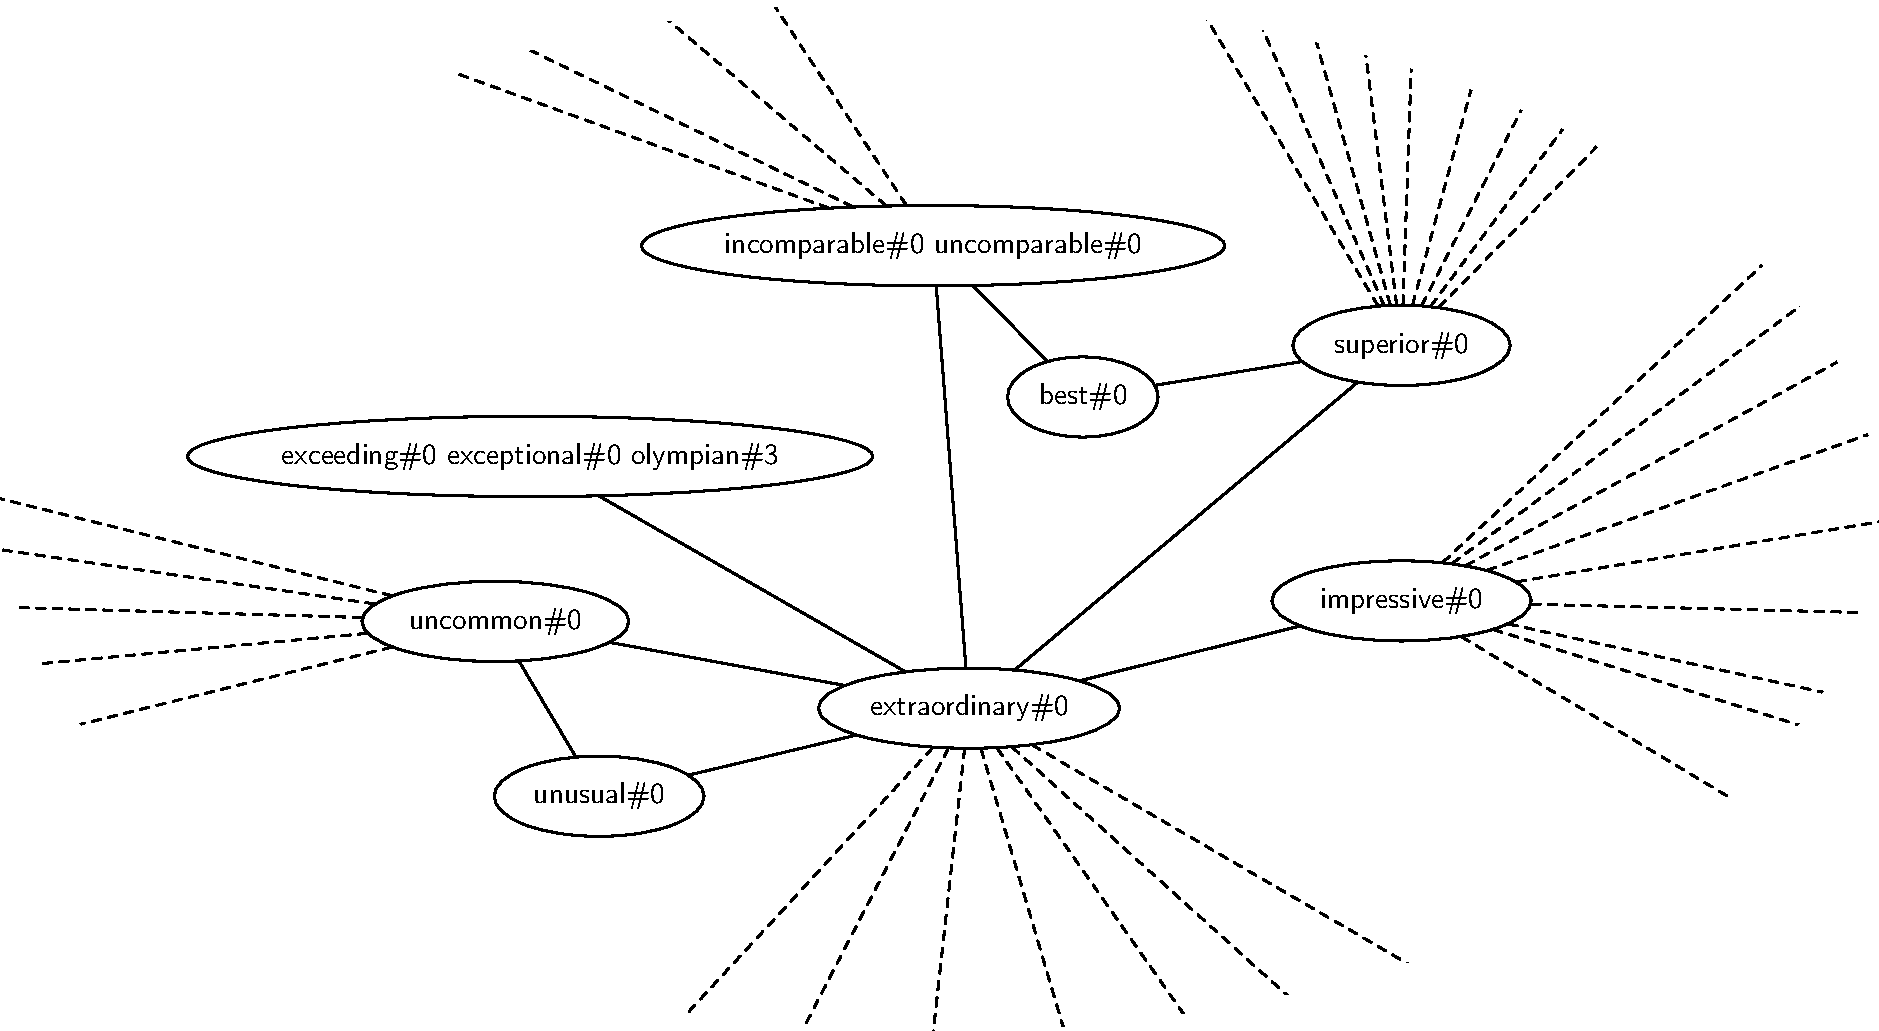
\includegraphics[scale=.27]{Figures/Exceptional}
  \caption{Illustration of relation in a semantic network.}
  \label{fig:semanticNetwork}
\end{figure}

The concrete semantic network used is WordNet, originally presented by \citeauthor{wordnet} \shortcite{wordnet}, and later presented in depth by \citeauthor{wordnetBook} \shortcite{wordnetBook}. Like it was the issue when acquiring a lexicon for the syntactic analysis, the availability of free semantic networks is very sparse. It has not been possible to find other competing networks with a coverage close to that of WordNet, and thus the decision of using WordNet is really based on it being the only choice. With that said, it is argued that WordNet is a quite extensive semantic network, which in its most recent revision (3.0) contains a relatively large number of semantic concepts, namely $|S| \approx \num{117000}$, while the number of lexical units recognized may be argued is not as covering as ideally, namely $|L| \approx \num{155000}$.

WordNet contains a variety of relations, $R$, however for the purpose of calculating sentiment polarity values, only the following were considered interesting:
\begin{itemize}
	\item The \emph{similar}-relation, $r_\mathrm{similar}$, links \emph{closely similar} semantic concepts, i.e.\ concepts having almost the synonymies mensing in most contexts. The relation is present for most concepts entailed by adjectives.
	\item The \emph{see also}-relation, $r_\mathrm{see\text{-}also}$, links \emph{coarsely similar} semantic concepts, i.e.\ concepts having a clear different mensing, but may be interpreted interchangeably for some contexts. Figure~\vref{fig:semanticNetwork} shows an example of exactly the \emph{see also}-relation.
	\item The \emph{pertainym}-relation, $r_\mathrm{pertainym}$, links the adjectives from which a adverb was derived, e.g.\ \emph{extreme} is the pertainym of \emph{extremely}.
\end{itemize}
\vspace{1em}

\section{Sentiment polarity of adjectives}
\label{sec:sentimentAdj}
The approach used to calculate sentiment polarity values for adjectives is very similar to the one presented by \citeauthor{valenceShifting} \shortcite{valenceShifting}, namely a domain specific set of positive and negative \emph{seed concepts} are identified, respectively $S_\mathrm{pos}$ and $S_\mathrm{neg}$. Each semantic concept in the sets can be described by a lexical unit and the specific index for that lexical unit that entail the desired concept, e.g.\ as shown in (\ref{eq:s_pos}) and (\ref{eq:s_neg}).
\begin{align}
	S_\mathrm{pos} &= \left\{ \text{clean}\#1, \text{quiet}\#1, \text{friendly}\#1, \text{cheap}\#1 \right\} \label{eq:s_pos}\\
	S_\mathrm{neg} &= \left\{ \text{dirty}\#1, \text{noisy}\#1, \text{unfriendly}\#1, \text{expensive}\#1 \right\} \label{eq:s_neg}
\end{align}

The graph $G_\mathrm{adj}$, given by (\ref{eq:g_adj}), is considered to calculate the sentiment polarity change inflicted by the adjective. Notice that the graph includes both the \emph{similar}-relation and the \emph{see\ also}-relation, as is desired to be able to reason about as large a set of adjectives as possible, and thus both closely and coarsely related concepts are considered.
\begin{align}
	G_\mathrm{adj} = (S, r_\mathrm{similar} \cup r_\mathrm{see\text{-}also})
	\label{eq:g_adj}
\end{align}
 
Given an adjective with lemma $\ell \in \Sigma^\star$, the set of semantic concepts that this adjective may entail, $M(\ell)$, should provide the basis for the sentiment polarity change inflicted by the adjective. The overall approach is to base the polarity change on the \emph{distances} between the concepts yielded by $M(\ell)$ and the seed concepts in $G_\mathrm{adj}$. However, as the system only has very limited domain knowledge, namely $S_\mathrm{pos}$ and $S_\mathrm{neg}$, there are no sure way of choosing which of the semantic concepts yielded by $M(\ell)$ is the ``right'' interpretation of $\ell$. Considering all of the possible concepts yielded by $M(\ell)$ nigher seem like a sane choice, since this would evidently flatten the polarities and end in vague results. The method used to solve this semantic ambiguity follows from the rational assumption that adjectives stated in the texts presumably are to be interpreted within the domain given by the seed concepts. Thus concepts from $M(\ell)$ that are strongly related to one or more seed concepts should be preferred over weaklier related concepts. The solution is to select the $n$ \emph{closest} relations between $M(\ell)$ and respectively $S_\mathrm{pos}$ and $S_\mathrm{neg}$, thus reasoning greedily positively, respectively greedily negatively, about $\ell$. The \emph{multiset} of all distances to either seed set for some lemma $\ell$ is given by $D_\mathrm{adj}(\ell, S')$, where $S'$ is either $S_\mathrm{pos}$ or $S_\mathrm{neg}$ cf.\ (\ref{eq:dist_adj}), and where $d_\mathrm{adj}$ is the distance function for $G_\mathrm{adj}$. The sub-multiset of $D_\mathrm{adj}(\ell, S')$ which contains the minimal $n$ values is denoted $D^n_\mathrm{adj}(\ell, S')$.
\begin{align}
    D_\mathrm{adj}(\ell, S') = \left[ d_\mathrm{adj}(s, s') \; | \; s \in M(\ell), s' \in S' \right] & \hspace{2em} \text{where $S' \in \{ S_\mathrm{pos}, S_\mathrm{neg}$ \}}
	\label{eq:dist_adj}
\end{align}

Finally the sentiment polarity for an adjective with lemma $\ell$, denoted $p_\mathrm{adj}(\ell)$, is then given by the \emph{difference} of the sums of the $n$ minimal \emph{normalized distances} cf.\ (\ref{eq:p_adj}), where $N$ is a normalization factor, ensuring that $p_\mathrm{adj}(\ell) \in \left[-\omega; \omega \right]$. This follows the intuition, that positive adjectives are \emph{closer} to $S_\mathrm{pos}$ than $S_\mathrm{neg}$ and vice-verse.
\begin{align}
    p_\mathrm{adj}(\ell) =     	
    	\left( \sum_{j \in  D^n_\mathrm{adj}(\ell, S_\mathrm{neg}) } N \cdot j \right) -
		\left( \sum_{j \in  D^n_\mathrm{adj}(\ell, S_\mathrm{pos}) } N \cdot j \right)
	\label{eq:p_adj}
\end{align}

Clearly this intuition is only valid if $|S_\mathrm{pos}| \approx |S_\mathrm{neg}|$, or more precisely, the probability of some random semantic concept is close to a positive concept should be the same as the probability of it being close to a negative concept. %Furthermore it is assumed that $d_\mathrm{adj}$ is \emph{normalized} cf.\ (\ref{eq:d_adj}), i.e. it always yields a value, such that $p_\mathrm{adj}(\ell) \in \left[-\omega; \omega \right]$.
%\begin{align}
%    d_\mathrm{adj}(s, s') \in \left[0; \frac{\omega}{n \cdot k}\right]	&\hspace{4em} \text{where $k = |S_\mathrm{pos}| = |S_\mathrm{neg}|$}
%    \label{eq:d_adj}
%\end{align}

The semantic expression of an adverb with type $\tau_\alpha \to \tau_\alpha$ is given by $e_\mathrm{adj}(\ell)$ in (\ref{eq:e_adj}).
\begin{align}
	e_\mathrm{adj}(\ell) &=
    \lambda x . x_{\circ p_\mathrm{adj}(\ell)}
	\label{eq:e_adj}
\end{align}

The calculation of $p_\mathrm{adj}(\ell)$ can be generalized for any semantic graph $G$, given its distance function $d$, and sets of respectively positive and negative \emph{seed concepts} $S_\mathrm{p}$ and $S_\mathrm{n}$ cf.\ (\ref{eq:p}). This generalization will be convenient in a moment, and $p_\mathrm{adj}$ is trivially expressible in terms of $p$: $p_\mathrm{adj}(\ell) = N \cdot p(d_\mathrm{adj}, S_\mathrm{pos}, S_\mathrm{neg}, \ell)$.
\begin{align}
    p(d, S_\mathrm{p}, S_\mathrm{n}, \ell) =     	
    	\left( \sum_{j \in  D_d^n(\ell, S_\mathrm{n}) } j \right) -
		\left( \sum_{j \in  D_d^n(\ell, S_\mathrm{p}) } j \right)	
	\label{eq:p}
\end{align}
where:
\begin{align}
	D_d(\ell, S') = \left[ d(s, s') \; | \; s \in M(\ell), s' \in S' \right] 
	\label{eq:p}
\end{align}

%The sentiment polarity for an adjective with lemma $\ell$ is denoted $p(G, S_\mathrm{pos}, S_\mathrm{neg}, \ell)$, where $G$ is the semantic graph, and $S_\mathrm{pos}, S_\mathrm{neg}$ are  cf.\ (\ref{eq:p_dcl})

\section{Sentiment polarity of adverbs}
\label{sec:sentimentAdverb}
The approach for calculating sentiment polarity values for adverbs is very similar to the approach used for adjectives. In fact, since WordNet does not define neither $r_\mathrm{similar}$ nor $r_\mathrm{see\text{-}also}$ on adverbs the basic approach is simply to lookup the adjective from which the adverb is derived from, if any, using $r_\mathrm{pertainym}$. However since adverbs might also \emph{intensify} or \emph{qualify} the meaning of a verb, adjective, or another adverb, some special treatment are presented for this. Analog to the positive and negative concepts, sets of respectively intensifying and qualifying seed adjectives are stated, e.g.\ (\ref{eq:s_itensify}) and (\ref{eq:s_qualify}).
\todo{Rethink those?}
\begin{align}
	S_\mathrm{intensify} &= \left\{ \text{extreme}\#1, \text{much}\#1, \text{more}\#1)\right\} \label{eq:s_itensify}\\
	S_\mathrm{qualify} &= \left\{ \text{moderate}\#1, \text{little}\#1, \text{less}\#1) \right\} \label{eq:s_qualify}
\end{align}

Recall from Section~\ref{sec:annotatingLexicon} that intensifiers and qualifiers are \emph{scaling} the value of the verb, adjective or adverb they modify. To calculate the factor of which an intensifier or qualifier inflicts, the graph $G_\mathrm{scale}$, given by (\ref{eq:g_scale}), is considered. The graph only contains the \emph{similar}-relation, since related intensifiers, respectively qualifiers, seem to be captured most precisely by only considering \emph{closely similar} adjectives to the selected seeds cf.\ \cite{valenceShifting}. Also notice that, unlike $S_\mathrm{pos}$ and $S_\mathrm{neg}$, these sets does not rely on the domain, as they only strengthens or weakens domain specific polarities. 
\begin{align}
	G_\mathrm{scale} = (S, r_\mathrm{similar})
	\label{eq:g_scale}
\end{align}

%The distance function for $G_\mathrm{scale}$, denoted $d_\mathrm{scale}$ is normalized such that the polarity of the adverb is in the range $[-1; 1]$ cf.\ (\ref{eq:d_scale}).
%\begin{align}
%    d_\mathrm{scale}(s, s') \in \left[0; \frac{1}{n \cdot k}\right]	&\hspace{4em} \text{where $k = |S_\mathrm{intensify}| = |S_\mathrm{qualify}|$}
%    \label{eq:d_scale}
%\end{align}

The value of a polarity scaling is then given by the exponential function (\ref{eq:p_scale}) with range $\left[\frac{1}{2}; 2 \right]$, i.e. the value of $p(d_\mathrm{scale}, S_\mathrm{intensify}, S_\mathrm{qualify}, \ell)$ is normalized using $N$ such it yields the range $[-1; 1]$. Thus a strong intensifier can double the sentiment polarity value of the unit it modifies, analogously a strong qualifier can reduce it by half.  
\begin{align}
    p_\mathrm{scale}(\ell) = 2^{N \cdot p(d_\mathrm{scale}, S_\mathrm{intensify}, S_\mathrm{qualify}, \ell)}
    \label{eq:p_scale}
\end{align}

Whether an adverb is considered and intensifier/qualifier or an normal adverb is determined by the value of $p_\mathrm{scale}(\ell')$, where $\ell'$ is the pertainym of the adverb. The semantic expression of an adverb with type $\tau_\alpha \to \tau_\alpha$ is given by $e_\mathrm{adverb}(\ell)$ in (\ref{eq:e_adverb}). If $p_\mathrm{scale}(\ell') \neq 1$ then the adverb is considered as a intensifier/qualifier and scales the lexical unit it inflicts, otherwise if the adverb is an derivation of an adjective it simply changes the inflicted unit with the value of the adjective. Finally the adverb can be one of a small set of predefined negatives, $L_\mathrm{neg}$, in this case the polarity of the inflicted unit is flipped. Otherwise the adverb is discarded by simply being annotated with the identity function.
\begin{align}
	e_\mathrm{adverb}(\ell) &=
	\begin{cases}    
    \lambda x . x_{\bullet p_\mathrm{scale}(\ell')} & \text{if $M(\ell) \times M(\ell') \subset r_\mathrm{pertainym}$ and $p_\mathrm{scale}(\ell') \neq 1$} \\
    \lambda x . x_{\circ p_\mathrm{adj}(\ell')} & \text{if $M(\ell) \times M(\ell') \subset r_\mathrm{pertainym}$} \\
    \lambda x . x_{\bullet -1} & \text{if $\ell \in L_\mathrm{neg}$}\\
    \lambda x . x & \text{otherwise}
	\end{cases}
	\label{eq:e_adverb}
\end{align}

\section{Completing the analysis}
All the components needed in order to calculate the sentiment of a text 
  \begin{align}
	 \mathcal{A}: \Sigma^\star \to S \to [-\omega;\omega] \tag{\ref{eq:Analysis}}	 
  \end{align}
% with the obvious exception that the distance function used of cause is with respect to $G_\mathrm{scale}$, and not $G_\mathrm{adj}$.
%!TEX root = Thesis.tex

\chapter{Implementation}
\label{chap:implementation}

It was chosen to use the functional programming language \emph{Haskell} for implementing the \emph{proof of concept} program. In the following sections key aspects of the implementation will be presented. For the complete source code for the implementation please see appendix~\ref{code}.

The reason Haskell, specifically the \emph{Glasgow Haskell Compiler}, was chosen as programming language and platform, was the ability to ... 
\clearpage

\cite{cs}

\section{WordNet interface}
The interface used to lookup data in WordNet is ... yada yada

However the interface is not complete ... the function for calculating the closure of synsets $S$ for some relatrion $R$ does not terminate if $R$ is symmetric. Since several semantic relations are symmetric (e.g. synonyms, antonyms)
%!TEX root = Thesis.tex

\chapter{Evaluation}
\label{chap:evaluation}


The data set used for evaluating the presented logical approach for sentiment analysis, specifically the \emph{proof of concept} system is the \emph{Opinosis Dataset}, originally used by \cite{Opinosis}. The data set consists of texts from actual user reviews on a total of 51 different topics. The topics are ranging over different objects, from consumer electronics (e.g.\ GPS navigation, music players, etc.) to hotels, restaurants and cars. For most of the objects, reviews are covered by multiple topics. For instance a specific car is covered by the topics \emph{comfort}, \emph{interior}, \emph{mileage}, \emph{performance}, and \emph{seats}.

It has been hard to find any real alternatives for the \emph{Opinosis Dataset} for several reasons: Most collected reviews are commercial, and thus not free to use; furthermore the \emph{Opinosis Dataset} also contains summerized texts for each of its topics, which are constructed by manual, human interpretation. The latter allow a straight approach for comparison of any results the proposed system will yield.\\
\begin{align}
  &\textit{The hotel buffet had fabulous food.}
  \label{txt:Ex1} \\[3mm]  
  &\textit{Very friendly servers and nice selection of food at a reasonable price.}
  \label{txt:Ex2} \\[3mm]  
  &\textit{Room service was extortionate though, very very expensive,} \nonumber \\
  &\textit{so we didnt bother, as food outlets a few minutes walk away.}
  \label{txt:Ex3}
\end{align}

The texts (\ref{txt:Ex1}) to (\ref{txt:Ex3}) show actual extracts from the data set for a topic on food quality on the Swissôtel Restaurant. While (\ref{txt:Ex1}) is a valid declarative sentence, (\ref{txt:Ex2}) is not, since it lacks a subject (i.e.\ the restaurant). A coarse review of the text in the dataset reveals that missing subjects are a repeating issue. This might not seem that odd, since many people would implicitly imply the subject from the topic that they are reviewing. Thus text missing subjects can in many cases still be considered as valid sentences with minimal effort. The text (\ref{txt:Ex3}) is on the other hand missing a transitive verb (presumably \emph{are}) from the subordinate clause. In cases where such savere gramatically errors occurs it is sugested to ignore the clause, and try only to analyse the main clause. Furthermore the text (\ref{txt:Ex3}) use repeated adverbs (e.g.\ \emph{very very}) to express intensification, however it should not be any major concern that a verb or adjective are modified multiple times by the \emph{same} adverb, but the intended intensification will probably not be included in the semantic analysis. Thus formalizing such a grammer is mostly a tak od designing such lexicon.

As evendent from these examples far from all texts in the dataset are valid sentences.

%!TEX root = Thesis.tex

\chapter{Conclusion}
\label{chap:Conclusion}

\section{Discussion}
Even though the stucture of the sentences is inspected deeply though the syntactic analysis the semantic expression assigned to adjectives and adverbs is still atomic, and based on the key concepts the the context specific positive and negative lists. Even though the lists are context specific, a concept can have ... løses dette evt. af subject-focus?


Since adjectives and adverbs are always reduced to only contribute to the polarity, they cannot be used to identify subjects. E.g. what do you think about the white iPhone vs. the black? (need bette ex.!)
\appendix
%!TEX root = Thesis.tex
\chapter{Appendix A}

\section{A naive attempt for lexicon acquisition}

\subsection{The Brown Corpus}
The Brown Corpus was compiled by \citeauthor{brown} \shortcite{brown} by collecting written works printed in United States during the year 1961. The corpus consists of just over one million words taken from 500 American English sample texts, with the intension of covering a highly representative variety of writing styles and sentence structures.

Notable drawbacks of the Brown Corpus include its age, i.e.\ there are evidently review topics where essential and recurring words used in present day writing was not coined yet or rarely used back 50 years ago. For instance does the Brown Corpus not recognize the words \emph{internet}, \emph{hotspot}

   sentences will containing words has found it's way into comon  that 

Other corpora has been considered

\section{Tokenizer and tagger}
The tokenizer has a very simple task, namely to convert an input string to a list of tokens (lower case words) that represent the symbols of the language. An example of the transformation is shown in
(\ref{fig:Tokenizer}).
\begin{align}
  &\text{``Put the pyramid onto the table.''} \to 
  \left[ 
  \token{put}, \token{the}, \token{pyramid}, \token{onto}, \token{the}, \token{table} 
  \right] 
  \label{fig:Tokenizer}
\end{align}

\subsection{Shift-reduce parser}
\section{Find a good title}
The initial attempt is simply to construct a parser that 

\begin{quote}
	There are three basic ways to build a shift-reduce parser. Full LR(1) (the `L' is the direction in which the input is scanned, the `R' is the way in which the parse is built, and the `1' is the number of tokens of lookahead) generates a parser with many states, and is therefore large and slow. SLR(1) (simple LR(1)) is a cut-down version of LR(1) which generates parsers with roughly one-tenth as many states, but lacks the power to parse many grammars (it finds conflicts in grammars which have none under LR(1)).
\end{quote}

\begin{quote}
LALR(1) (look-ahead LR(1)), the method used by Happy and yacc, is tradeoff between the two. An LALR(1) parser has the same number of states as an SLR(1) parser, but it uses a more complex method to calculate the lookahead tokens that are valid at each point, and resolves many of the conflicts that SLR(1) finds. However, there may still be conflicts in an LALR(1) parser that wouldn't be there with full LR(1).
\end{quote}

The state $S_\tau$ ...

Formally a rule $\mathcal{R}_\tau$, for the state type $\tau$, is a transformation from a state $s \in \mathcal{S}_\tau$ onto a new set of states $\mathcal{S}_\tau' \subset \mathcal{S}_\tau$ cf. \ref{eq:Rule}.
\begin{equation}
	\mathcal{R}_\tau : \mathcal{S}_\tau \to \mathcal{P}(\mathcal{S}_\tau)
	\label{eq:Rule}
\end{equation} 

The state type for analysing CCGs is a 2-tuple, where $P$ is  a totally ordered set of ..., 

$$\mathcal{S}_\mathrm{CCG} : \mathcal{P}(T) \times \mathcal{P}(\mathcal{P}(T))$$

\begin{equation}
	\mathcal{R}^\mathrm{shift}_\mathrm{CCG}
\end{equation}

If all rules in the set is monotone, then the parsing will terminate 

							              %Appendix A
%-----------
% Backmatter
%-----------
\backmatter
\chaptermark{Bibliography}
\renewcommand{\sectionmark}[1]{\markright{#1}}
\sectionmark{Bibliography}
\addcontentsline{toc}{chapter}{Bibliography}        %Force addition of Bibliography to TOC
\bibliographystyle{named}                           %Use alpha codes for references
\bibliography{References}    	                      %Bibliography file called
\end{document}
% % % EOF % % %